\documentclass[11pt]{article}
\usepackage[margin=1in]{geometry}
\usepackage{setspace}
\onehalfspacing
\usepackage[bottom]{footmisc}
\usepackage{amsmath, amssymb, amsthm}
\usepackage{mathtools}
\usepackage{booktabs}
\usepackage{array}
\usepackage{graphicx}
\usepackage{tikz}
\usetikzlibrary{arrows.meta}
\usepackage[section]{placeins}
\renewcommand{\topfraction}{0.9}
\renewcommand{\bottomfraction}{0.85}
\renewcommand{\textfraction}{0.08}
\renewcommand{\floatpagefraction}{0.75}
\setcounter{topnumber}{3}
\setcounter{totalnumber}{6}
\usepackage[round,authoryear]{natbib}
\bibpunct{(}{)}{;}{a}{}{,}
\setlength{\bibsep}{2pt}
\usepackage[hidelinks]{hyperref}
\newtheorem{proposition}{Proposition}
\numberwithin{proposition}{section}
\newtheorem{corollary}[proposition]{Corollary}
\newtheorem{lemma}[proposition]{Lemma}
\theoremstyle{definition}
\newtheorem{assumption}{Assumption}
\theoremstyle{remark}
\newtheorem*{remark}{Remark}
\theoremstyle{plain}
\newcommand{\R}{\mathbb{R}}
\newcommand{\E}{\mathbb{E}}
\newcommand{\sstock}{\mathrm{SS}}

\title{Cost, Carbon, and the Speed of Replenishment\\ in Distribution Network Design}
\author{}
\date{}

\begin{document}
\maketitle

\begin{abstract}
\noindent Firms that distribute through regional distribution centers need to reconsider how many centers to operate and
how fast to replenish them as carbon is increasingly priced into these decisions, whether voluntarily by the firm
or through regulation. In this paper, we examine which way, and how far, a carbon price or cap moves the two
decisions. Each decision
trades one source of emissions against another. Slower line haul burns less fuel but requires more safety stock
and more stock in transit; more distribution centers shorten the last mile but add buildings and give up the
pooling that keeps inventory low. We model the two decisions jointly and show that the design problem has a
unique optimum at every carbon price. For a given network, carbon pricing favors faster replenishment when the
inventory that speed saves emits more per dollar than the speed itself. Goods in transit carry a financing cost
but no carbon: for a given network, financing them raises the cost-minimizing speed without changing the
carbon-minimizing speed. For a given speed, carbon pricing favors more
distribution centers when a dollar of last-mile delivery emits more than a dollar of facilities and lost pooling.
With both decisions adjustable, a small carbon price can favor consolidation even when the carbon-minimizing
network is more dispersed. A firm can compute these comparisons from its operating rates, demand characteristics,
and cost-minimizing configuration.
\end{abstract}

\vspace{1em}
\noindent\textbf{Keywords:} Distribution network design; Carbon pricing; Replenishment speed; Safety stock; Last-mile delivery; Continuous approximation

\newpage

\section{Introduction}\label{sec:intro}

How many distribution centers to operate and how fast to replenish them are long-standing questions in
distribution network design \citep{eppen1979effects, daskin2002inventory, shen2003joint}, and firms continue to
revisit both. Some have moved stock closer to demand. Amazon divided its US fulfillment network into eight
regions and reported a $19\%$ reduction in the miles traveled to deliver packages \citep{amazon2023q2}, and Home
Depot is building flatbed distribution centers in its forty largest markets \citep{homedepot2020fdc}. Others
have slowed their line haul. AstraZeneca has moved most of its international freight from air to ocean and ships
about $65\%$ of its cargo by sea \citep{pharmcommerce2023astrazeneca}, and truckload shippers typically convert
lanes to intermodal rail once the savings reach $10$ to $15\%$ \citep{freightwaves2026intermodal}. The reasons
these firms give are mainly cost and delivery service; Amazon also describes shorter shipments as better for the
environment, and AstraZeneca relates its shift to its sustainability efforts. What is new is that carbon is
beginning to be priced and reported:
the European Union has priced the carbon of maritime shipping since 2024 \citep{eu2023ets} and will price road
fuel from 2028 \citep{eea2026ets2}. California is phasing in the reporting of supply-chain emissions from 2027
\citep{california2023sb253}, and ISO 14083 standardizes how the emissions of transport and warehouses are
counted \citep{iso2023_14083}. A firm that prices or caps its distribution carbon must therefore ask which way, and how far, a carbon price
moves these two decisions.

In this paper, we examine how a carbon price changes these two decisions: the \emph{density} of the network ---
how many distribution centers the firm operates --- and the \emph{speed} with which those centers are
replenished. Each decision trades one source of carbon against another. Slowing replenishment moves freight by
slower, lower-emission modes, as in slow steaming in shipping \citep{psaraftis2013speed, cariou2011slow}, but it
lengthens the lead time that safety stock must cover, so the safety stock, and the carbon of holding it, rises
with the square root of that lead time. Consolidating serves markets from fewer, larger distribution centers
\citep{mckinnon2012setting} and pools demand across markets \citep{eppen1979effects}; it saves facility energy
and inventory but lengthens the last mile. A firm thus provides \emph{availability} either by holding safety
stock or by replenishing faster, and market \emph{proximity} either by operating more local facilities or by
delivering farther from fewer. The cost-minimizing design uses one mix of these activities; with carbon priced,
the mix can change.

The direction of the change depends on carbon intensity per dollar. For a given network, the carbon-minimizing
chain replenishes \emph{faster} when the inventory that faster replenishment saves emits more per dollar than the
inbound transport that would replace it. For a firm that finances its goods in transit, faster replenishment saves capital as well as safety stock.
Capital carries no carbon, so financing raises the cost-minimizing speed without changing the carbon-minimizing
one. For a given speed,
the carbon-minimizing chain operates a \emph{more dispersed} network when last-mile travel emits more per dollar
than the facilities that would shorten it and the pooling they give up. 

We formalize this in a single-product location--inventory model with stochastic demand. The firm chooses network
density and replenishment speed to minimize cost subject to a cap on expected or realized carbon and a service requirement. The model follows the location--inventory tradition
\citep{daskin2002inventory, shen2003joint} in a continuous-approximation form \citep{daganzo2005logistics}, with
replenishment speed as a continuous decision. Because speed sets the lead time that safety stock must cover, it
links transport and inventory in both cost and carbon, and the continuous form lets us state in closed form how
pooling and the financing of goods in transit enter the comparison.

We contribute to the literature in three ways. First, we show how inventory pooling and the financing of goods
in transit shape the cost--carbon comparison. The design problem has a unique optimum at every carbon price. For a
given network, a carbon price favors faster replenishment only when the inventory that speed saves emits more per
dollar than the speed itself, and financing goods in transit works against it. For a given speed, the comparison
for density weighs the last mile against facilities and the pooling that an additional center gives up. When
speeds are interior, four carbon intensities per dollar and two shares of the cost-minimizing design, for lost
pooling and for safety stock, give the direction of density, and of speed when the two
comparisons agree. A price on transport carbon alone can raise total carbon, because it substitutes inventory and
facilities for transport even where they emit more per dollar than that transport. Second, we estimate the ratios
from public US data. Activities whose cost is mostly energy emit far more carbon per dollar than those whose cost
is mostly labor or capital, so the direction depends on how the firm buys speed and how it delivers the last
mile. At the central values, speed bought with fuel emits more per dollar than holding the stock of any product we
examine, so a carbon price favors slower replenishment; diesel delivery and electric trucks call for more distribution centers,
and electric vans for fewer in cold chains. Third, we illustrate the results in a reference network whose line-haul speeds correspond to truckload,
intermodal, and carload rail. When the firm finances its stock in transit, slower line haul delivers most of a
$20\%$ cut in emissions, changing both decisions costs less than slowing alone and reaches deeper cuts, and whole
facilities change the design little.

The paper is structured as follows. In Section~\ref{sec:related}, we position the paper in the literature. In
Section~\ref{sec:model}, we develop the model, and in Section~\ref{sec:analysis} we answer the questions a
firm asks of its network.
Section~\ref{sec:numerical} applies them to US data, Section~\ref{sec:managerial} draws out managerial
implications, and Section~\ref{sec:discussion} concludes.

\section{Related Literature}\label{sec:related}

Our work connects four streams of research: location--inventory design with risk pooling, carbon-aware network
design, the joint control of inventory and transport mode under emissions regulation, and carbon as a priced cost
in service-constrained inventory systems. Each develops part of the two substitutions we study --- availability
(inventory or replenishment speed) and proximity (facilities or last-mile travel). We draw on all four and add the
joint design of network density and replenishment speed under a carbon cap and a service requirement, a
classification of the direction in which carbon moves both decisions, and a calibration of the carbon intensities
that determine it.

\subsection{Location--inventory design and risk pooling}

A first stream establishes how demand risk pooling shapes distribution network design: jointly choosing
facility location and safety stock, it characterizes the cost-optimal number and placement of distribution
centers. \citet{eppen1979effects} characterizes the effect of centralization on expected cost in the
multi-location newsvendor, establishing the square-root relationship between the number of stocking locations
and pooled safety stock. \citet{daskin2002inventory} and \citet{shen2003joint} embed working and safety stock
into the facility-location decision, so that risk pooling shapes the optimal number and placement of
distribution centers, with extensions to stochastic settings by \citet{snyder2007stochastic}, to capacitated
warehouses by \citet{ozsen2008capacitated}, and to continuous-approximation allocation by
\citet{tsao2012continuous}. \citet{daganzo2005logistics} provides the continuous-approximation foundation in
which last-mile distance scales with the inverse square root of the number of facilities, and
\citet{blumenfeld1985analyzing} use continuous approximations to trade transportation against inventory and
production costs in choosing routes and shipment sizes on freight networks. Closest to our spatial--inventory
coupling, \citet{straubert2024continuous} ties the number of stocking locations to an exact
reorder-point/order-quantity inventory model through a delivery-lead-time penalty, solved by continuous
approximation. Recent work extends the location--inventory problem in directions close to ours. \citet{hu2025location} add the choice of storage temperature, and \citet{jalal2026integrated} integrate
multi-period location, inventory, and transportation decisions for a pharmaceutical network.
\citet{puttemans2025integration} review this literature. Beyond demand pooling, \citet{schmitt2015centralization} show that diversifying supply-disruption risk can
favor decentralization for a risk-averse firm. These works
develop network density and safety-stock placement under risk pooling with a cost or service objective. We retain
the risk-pooling structure and the density decision and add a replenishment speed chosen together with density,
and a carbon objective.

\subsection{Carbon-aware network design}

A second stream brings carbon into facility location and network design, characterizing how an emissions
objective or cap can change the optimal network configuration. \citet{cachon2014retail}
relates retail store density to greenhouse gas cost, with consumer travel to stores as the dominant emission
channel and inventory entering through retail floor space. \citet{turken2017facility} examine facility location
and capacity under a carbon tax and emission limits, weighing centralization against decentralization through
production scale economies, and \citet{harris2011assessing} compare cost-optimal and emissions-aware network
designs numerically. \citet{wang2020carbon} develop a carbon-compliant location--inventory model under demand and
carbon-price uncertainty, and \citet{li2017joint} jointly optimize distribution-network design and two-echelon
inventory under a CO\textsubscript{2} emission tax. \citet{bouchery2015cost} locate intermodal terminals and split
freight between direct trucking and intermodal transport, and trace the trade-off between cost and carbon that
modal shift creates. \citet{hacardiaux2020assessing, hacardiaux2022balancing} assess the emission savings of a
shared location--inventory network under horizontal cooperation and balance the partners' preferences over cost
and carbon. Closest to ours in method, \citet{zhang2026economic} combine continuous
approximation with integer programming to show how a carbon price reshapes the choice among drone,
truck--drone, and truck last-mile delivery.
These studies make density or facility configuration the central decision and bring emissions into the
objective, the constraints, or an ex post assessment; where transport is an operational choice, it enters through
travel distances, discrete modes, or lead-time parameters. We treat network density and replenishment speed as
joint decisions and characterize the proximity substitution between facilities and last-mile travel
analytically.

\subsection{Inventory, transport mode, and emissions}

A third stream couples transport-mode and lead-time choices with inventory control under emissions regulation,
characterizing how carbon reshapes the trade-off between freight and the inventory it serves. Its foundation is
the inventory-theoretic model of \citet{baumol1970inventory}, who value a freight service by its rate, speed, and
reliability through the stock in transit and the safety stock it requires.
\citet{hoen2014effect} and \citet{chen2016effects} study transport mode selection alongside
inventory under stochastic demand and emissions regulation; \citet{qi2022transport} select door-to-door transport
services and routes for China--Europe freight against transport cost, in-transit inventory cost, and carbon; \citet{bektas2011pollution} embed load-dependent fuel use and emissions in vehicle routing; \citet{moradi2025load} optimize driving speed and path
under load-dependent fuel use; \citet{konur2014integrated} solve the economic
order quantity model with less-than-truckload and truckload carriers under carbon cap, tax, and cap-and-trade
regulation, and \citet{schaefer2015economic} extend this to a continuous-review system under stochastic demand and trace the
cost--emission frontier. \citet{drent2023efficient} analyze dynamic dual supply-mode selection under an emission target,
and \citet{hammami2015carbon} bring carbon from manufacturing, ordering, and inventory into a multi-echelon
production--inventory model with lead-time constraints. In shipping, \citet{maloni2013slow} show by simulation
that slower vessel speed lowers both total cost and carbon on an Asia--North America lane while raising the pipeline inventory that shippers carry. Our speed threshold prices the carbon as well as the cost of
the inventory that slower replenishment requires, including the financing of stock in transit. In these papers,
transport service enters through route and load physics, carrier class, discrete supply modes, or lead-time
parameters and constraints. We add the speed and density thresholds that result when replenishment speed and
network density are chosen jointly under a carbon cap and a service requirement.

Closest in its combination of decisions, \citet{comasmarti2015carbon} design a supply chain network under
uncertain demand in which each market is assigned a manufacturing facility and one of four discrete transport
modes, with a continuous-review inventory policy at each market, the carrying cost of goods in transit, and caps
or taxes on carbon. They solve integer programs numerically and show that functional and innovative products call
for different networks and abatement, and that a carbon tax set at the marginal abatement cost achieves roughly
the abatement of the corresponding cap. In their model each market holds its own stock, and lead time follows from
the chosen mode and distance. We pool markets at distribution centers and treat replenishment speed as a
continuous decision, which gives closed-form conditions for the direction of both decisions and shows how pooling
and the financing of goods in transit enter them.
\citet{boone2025freight} choose a discrete freight mode against inventory under an emission cap at a single
location. We replace the finite set of modes with a continuous replenishment speed, price carbon on the holding
as well as the transport side, and embed the speed decision in a network whose density is chosen jointly.

\subsection{Carbon policy, service, and safety-stock placement}

A fourth stream prices carbon directly into inventory and service decisions, showing how a carbon price or cap
shifts order quantities and safety-stock placement.
\citet{hua2011managing} and \citet{bouchery2012including} develop carbon-aware order-quantity models under
cap-and-trade and multi-objective formulations, and \citet{benjaafar2013carbon} position cap, tax, and
cap-and-trade as priced operational instruments in simple supply-chain models; \citet{chen2013carbon} derive the
closed-form carbon-constrained economic order quantity, the single-location analog of the marginal
carbon-intensity logic we extend to a network, and \citet{arikan2014single} impose a product carbon-footprint
constraint on a dual-sourcing newsvendor. \citet{silbermayr2017inventory} bring environmental constraints into
inventory pooling with dependent demand. Within multi-echelon service models,
\citet{ni2015tradeoff} study the trade-off between service time and carbon in safety-stock placement under the
guaranteed-service framework, and \citet{wang2025inventory} incorporate cap-and-trade into guaranteed-service
placement. Probabilistic carbon limits have been modeled through chance constraints in lot sizing
\citep{koca2021stochastic} and in supply-chain network design \citep{shaw2016low}, typically inside large
mixed-integer programs; our deterministic equivalent scales the transport component of carbon by a single factor. \citet{sebatjane2025sustainable} survey these models. The service-placement models price carbon against service and
safety stock; we add network density and replenishment speed. 
\section{The Model}\label{sec:model}

\subsection{Operational environment}

\paragraph{Region and markets.} A firm serves $N$ markets distributed over a service region of area $A$.
Per-period demand at market $i$ is a random variable with mean $\mu$ and standard deviation $\sigma$,
identically distributed across markets with common pairwise correlation $\rho \in [0,1)$. Demand is
stationary and the setting is single-product. Markets and distribution centers are treated symmetrically, the standard
simplification that admits closed-form continuous-approximation results \citep{daganzo2005logistics}.

\paragraph{Distribution centers and geography.} The firm opens $n$ identical distribution centers (DCs), $1 \le n \le N$, each
serving a sub-region of area $A/n$. By the continuous-approximation spatial law, the mean last-mile
(DC-to-market) distance falls as the square root of the served area,
\begin{equation}\label{eq:dn}
  d(n) \;=\; \delta\, n^{-1/2}, \qquad \delta \propto \sqrt{A},
\end{equation}
so a denser network shortens delivery but only at a decreasing rate \citep{daganzo2005logistics}.

\paragraph{Replenishment and the speed decision.} Each DC is replenished directly from the source at a chosen
speed $v \in [v_{\min}, v_{\max}]$. Individual DCs lie at different distances from the source; what enters
cost and carbon is total inbound freight: with identical DCs each carrying throughput $N\mu/n$, this is
$\sum_j (N\mu/n)\,D_j = N\mu\,\bar D$, the total throughput times the \emph{mean} source-to-DC distance
$\bar D$. Because the DCs fill a region of fixed
size served from a fixed source, $\bar D$ is set by the region's geometry (order $\sqrt A$) and is
approximately invariant to $n$; we set $D \equiv \bar D$ and treat it as constant.\footnote{Two
modeling reductions are embedded here. First, the symmetric-DC reduction assigns every DC the representative lead
time $L = \bar D/v$ in place of its own $L_j = D_j/v$. Safety stock enters through $\sqrt{L}$, which is
concave in distance, so by Jensen's inequality $\sqrt{\bar D} \ge n^{-1}\sum_j \sqrt{D_j}$
\citep{jensen1906fonctions}: using the mean distance slightly \emph{overstates} aggregate safety stock, by a
gap that is second-order in the dispersion of the $D_j$ and reduces as the distances equalize. Second, replenishment is
point-to-point; on a consolidated route the inbound distance would grow as $\sqrt{n}$, as in the store-delivery
tour of \citet{cachon2014retail}, which reinforces centralization.}
The replenishment lead time is then
\begin{equation}\label{eq:lead}
  L(v) \;=\; D/v .
\end{equation}
Lead time is the only channel through which speed affects inventory: safety stock covers demand over the lead
time, and the goods in transit are proportional to it. Shortening the lead time is not free. We use $t(v)$ and
$\varepsilon(v)$ to denote the cost and carbon of inbound freight per unit-mile at speed $v$, and we assume only
that both increase with $v$ and are convex; for the closed-form results, we use the quadratic instantiation
$\varepsilon(v)=\varepsilon_b+\varepsilon_0 v^2$ and $t(v)=t_0+t_1 v^2$, with intercepts $\varepsilon_b\ge0$ and
$t_0$ that do not vary with speed, the canonical form motivated by the cubic fuel-speed
law of slow steaming \citep{psaraftis2013speed, cariou2011slow}. On a given origin--destination lane, a
faster mode such as truckload instead of intermodal rail, a faster vessel, or a team of two drivers who keep the
truck moving all deliver a shorter lead time at a higher freight cost, and they differ in how much of that cost is
fuel.

\paragraph{Fuel and other costs of replenishment.} We divide the transport cost rate into fuel and other costs,
$t(v)=t^{\mathrm f}(v)+t^{\mathrm o}(v)$. With a fixed
fuel price and emission factor, and with fuel accounting for the emissions that vary with speed,
$\varepsilon'(v)=\chi_{\mathrm f}\,t^{\mathrm f\prime}(v)$, where $\chi_{\mathrm f}$ is the carbon per dollar of fuel, so that
\begin{equation}\label{eq:rtfuel}
  \frac{\varepsilon'(v)}{t'(v)}=\chi_{\mathrm f}\,\xi(v),\qquad \xi(v)=\frac{t^{\mathrm f\prime}(v)}{t'(v)}.
\end{equation}
When both cost components rise with speed, $\xi(v)$ is the fuel share of the marginal cost of speed. Under the
quadratic instantiation, $t_1=b_{\mathrm f}+b_{\mathrm o}$ and $\varepsilon_0=\chi_{\mathrm f} b_{\mathrm f}$, where $b_{\mathrm f}v^2$ and $b_{\mathrm o}v^2$ are the
speed-dependent fuel and other costs, so that $\varepsilon_0/t_1$ is constant. Moving from intermodal rail to truckload shortens lead time by burning more fuel per unit-mile, so most of its
added cost is fuel. A team of two drivers shortens lead time at nearly the same fuel, and so nearly the same
carbon, per mile, so most of its added cost is the second driver's wages. Where $t$ is a freight rate, the relation assumes that fuel costs pass through to the
rate.

\begin{figure}[b]
\centering
\begin{tikzpicture}[x=0.52pt, y=-0.52pt,
  region/.style={rounded corners=5pt, draw=black!45, thin},
  part/.style={draw=black!45, thin, dash pattern=on 4pt off 3pt},
  dcbox/.style={draw=black!55, fill=black!8, rounded corners=2pt, thin},
  stock/.style={fill=black!40},
  spoke/.style={line width=0.45pt, draw=black!85},
  llink/.style={line width=1.0pt, draw=black, -{Stealth[length=5pt]}},
  mkt/.style={circle, fill=black, inner sep=0pt, minimum size=4.4pt},
  lbl/.style={font=\scriptsize, inner sep=1pt},
  wlbl/.style={font=\scriptsize, inner sep=1pt, fill=white},
  pcap/.style={font=\footnotesize, inner sep=1pt}]
\draw[region] (45,45) rectangle (345,345);
\draw[part] (195,46) -- (195,344);
\foreach \p in {(83,90),(150,78),(70,160),(78,280),(140,310),(172,250)} \draw[spoke] (113,192) -- \p;
\foreach \p in {(242,85),(308,100),(322,165),(312,278),(252,308),(218,255)} \draw[spoke] (277,192) -- \p;
\node[wlbl] at (80,244) {$d(2)$};
\draw[dcbox] (92,172) rectangle (134,212);
\node[lbl] at (113,181) {DC 1};
\foreach \yy in {188,196,204} \fill[stock] (102,\yy) rectangle +(22,6);
\draw[dcbox] (256,172) rectangle (298,212);
\node[lbl] at (277,181) {DC 2};
\foreach \yy in {188,196,204} \fill[stock] (266,\yy) rectangle +(22,6);
\fill[black, rounded corners=2pt] (170,177) rectangle (220,197);
\node[lbl, text=white] at (195,187) {Source};
\draw[llink] (170,187) -- (138,190);
\node[wlbl] at (152,174) {$L$};
\draw[llink] (220,187) -- (252,190);
\node[wlbl] at (238,174) {$L$};
\foreach \p in {(83,90),(150,78),(70,160),(78,280),(140,310),(172,250),(242,85),(308,100),(322,165),(312,278),(252,308),(218,255)} \node[mkt] at \p {};
\node[pcap] at (195,367) {$n=2$: each DC serves 6 markets};
\node[pcap, text=black!60] at (195,385) {more stock per DC, longer delivery legs};
\begin{scope}[shift={(370,0)}]
\draw[region] (45,45) rectangle (345,345);
\draw[part] (195,46) -- (195,344);
\draw[part] (46,195) -- (344,195);
\foreach \p in {(83,90),(150,78),(70,160)} \draw[spoke] (140,119) -- \p;
\foreach \p in {(242,85),(308,100),(322,165)} \draw[spoke] (250,119) -- \p;
\foreach \p in {(78,280),(140,310),(172,250)} \draw[spoke] (140,255) -- \p;
\foreach \p in {(312,278),(252,308),(218,255)} \draw[spoke] (250,255) -- \p;
\node[wlbl] at (95,132) {$d(4)$};
\draw[dcbox] (119,102) rectangle (161,136);
\node[lbl] at (140,111) {DC 1};
\foreach \yy in {118,126} \fill[stock] (129,\yy) rectangle +(22,6);
\draw[dcbox] (229,102) rectangle (271,136);
\node[lbl] at (250,111) {DC 2};
\foreach \yy in {118,126} \fill[stock] (239,\yy) rectangle +(22,6);
\draw[dcbox] (119,238) rectangle (161,272);
\node[lbl] at (140,247) {DC 3};
\foreach \yy in {254,262} \fill[stock] (129,\yy) rectangle +(22,6);
\draw[dcbox] (229,238) rectangle (271,272);
\node[lbl] at (250,247) {DC 4};
\foreach \yy in {254,262} \fill[stock] (239,\yy) rectangle +(22,6);
\fill[black, rounded corners=2pt] (170,177) rectangle (220,197);
\node[lbl, text=white] at (195,187) {Source};
\draw[llink] (183,177) -- (158,142);
\node[wlbl] at (163,162) {$L$};
\draw[llink] (207,177) -- (232,142);
\node[wlbl] at (227,162) {$L$};
\draw[llink] (183,197) -- (158,232);
\draw[llink] (207,197) -- (232,232);
\foreach \p in {(83,90),(150,78),(70,160),(78,280),(140,310),(172,250),(242,85),(308,100),(322,165),(312,278),(252,308),(218,255)} \node[mkt] at \p {};
\node[pcap] at (195,367) {$n=4$: each DC serves 3 markets};
\node[pcap, text=black!60] at (195,385) {less stock per DC, shorter delivery legs};
\end{scope}
\node[pcap, font=\footnotesize\bfseries] at (380,418) {Faster replenishment (shorter $L$), at a given density:};
\node[pcap] at (380,436) {system-wide safety stock shrinks, so holding cost and carbon fall, while freight cost and carbon rise.};
\node[pcap, font=\footnotesize\bfseries] at (380,462) {More DCs (higher $n$), at a given speed:};
\node[pcap] at (380,480) {delivery legs $d(n)$ shorten with territory area, so system-wide last-mile cost and carbon fall,};
\node[pcap] at (380,496) {while facility cost and carbon rise and weaker pooling raises system-wide holding cost and carbon.};
\end{tikzpicture}
\caption{Model representation for 12 markets ($N$) and 2 or 4 DCs ($n=2$ or $4$).}
\label{fig:setting}
\end{figure}

\paragraph{Inventory and service.} Each DC operates a base-stock policy and must meet a cycle service level
$\alpha$, the in-stock probability at the end of a period. With normally distributed demand the safety factor is $z = \Phi^{-1}(\alpha)$, with $\alpha>\tfrac12$ so
that $z>0$, taken here as a service requirement (a parameter). Demand is independent across periods, and each DC reviews its
inventory continuously, so safety stock protects against demand over the replenishment lead time; under periodic
review the protection interval would also include the review period. A DC that pools $g = N/n$ markets faces aggregate per-period demand with
standard deviation $\sigma\sqrt{g\,[\,1+(g-1)\rho\,]}$, the statistical economy of scale in inventory
\citep{eppen1979effects}. Covering lead-time demand, each DC holds safety stock
$z\,\sigma\sqrt{L}\,\sqrt{g[1+(g-1)\rho]}$. Summing over the $n$ DCs and defining the \emph{pooling expression}
\begin{equation}\label{eq:psi}
  \Psi(n) \;=\; N\rho + n(1-\rho),
\end{equation}
the system-wide safety stock is
\begin{equation}\label{eq:ss}
  \sstock(n,v) \;=\; z\,\sigma\,\sqrt{D/v}\;\sqrt{N\,\Psi(n)} .
\end{equation}
At $\rho = 0$, \eqref{eq:ss} reduces to $z\sigma\sqrt{L}\sqrt{nN}$, the square-root law: decentralizing
from $1$ to $N$ DCs multiplies safety stock by $\sqrt{N}$. As $\rho \to 1$, $\Psi(n) \to N$ and safety stock
becomes invariant to $n$.

\paragraph{Decisions.} The firm chooses the network density $n \in [1,N]$ (relaxed to a continuous
variable) and the replenishment speed $v \in [v_{\min}, v_{\max}]$. Table~\ref{tab:notation} collects the notation.

\begin{table}[t]
\centering\small
\caption{Notation. The decision variables are the network density $n$ and the replenishment speed $v$;
all other quantities are exogenous parameters or derived.}
\label{tab:notation}
\begin{tabular}{@{}>{\itshape}l p{0.70\linewidth}@{}}
\toprule
\textbf{Symbol} & \textbf{Meaning} \\
\midrule
\multicolumn{2}{@{}l}{\textbf{Decision variables}}\\
\;\;$n$ & number of DCs (network density), $1\le n\le N$\\
\;\;$v$ & replenishment speed, $v\in[v_{\min},v_{\max}]$\\
\addlinespace
\multicolumn{2}{@{}l}{\textbf{Demand (exogenous)}}\\
\;\;$N$ & number of markets\\
\;\;$\mu,\ \sigma$ & mean, standard deviation of demand per market per period\\
\;\;$\rho$ & cross-market demand correlation, $\rho\in[0,1)$\\
\addlinespace
\multicolumn{2}{@{}l}{\textbf{Geography, cost, carbon (exogenous)}}\\
\;\;$A,\ D,\ \delta$ & region area; inbound distance; last-mile distance constant\\
\;\;$F,\ \varphi$ & fixed cost, carbon per DC per period\\
\;\;$c$ & handling cost per unit handled\\
\;\;$h,\ \eta$ & holding cost, carbon per unit per period\\
\;\;$h_p$ & financing cost of stock in transit per unit per period\\
\;\;$t(v),\ \varepsilon(v)$ & inbound transport cost, carbon per unit-mile (convex in $v$)\\
\;\;$t_L,\ \varepsilon_L$ & last-mile transport cost, carbon per unit-mile\\
\;\;$\alpha$ & cycle service level (in-stock prob.); $z=\Phi^{-1}(\alpha)$\\
\;\;$\tau,\ B$ & carbon price; carbon cap\\
\addlinespace
\multicolumn{2}{@{}l}{\textbf{Derived}}\\
\;\;$g=N/n$ & markets served per DC\\
\;\;$L=D/v$ & replenishment lead time\\
\;\;$d(n)=\delta\,n^{-1/2}$ & mean last-mile distance\\
\;\;$\Psi(n)=N\rho+n(1-\rho)$ & pooling expression\\
\;\;$\sstock(n,v)$ & system-wide safety stock, eq.~\eqref{eq:ss}\\
\;\;$P(v)=N\mu D/v$ & stock in transit\\
\;\;$a(n,v)$ & safety-stock share of the inventory saving from speed, eq.~\eqref{eq:stockshare}\\
\bottomrule
\end{tabular}
\end{table}

\subsection{Cost and carbon}

Both the cost and carbon functions are system-wide flows over a single
representative period, consistent with the stationary single-product environment above:
$F,\varphi$ are charged per DC per period, $h,\eta$ per unit held per period, and the transport terms accrue
against the per-period throughput. The representative distances in Figure~\ref{fig:setting} therefore enter
global cost and carbon through aggregate freight tasks, not through a per-territory objective. Throughput
itself is conserved at $N\mu$ regardless of the configuration: the firm moves the mean demand of all $N$
markets through the network, whatever density $n$ and speed $v$ it chooses. With per-period throughput
$N\mu$,
\begin{align}
  K(n,v) &= \underbrace{F\,n+c\,N\mu}_{\text{facilities}} + \underbrace{h\,\sstock(n,v)}_{\text{holding}} + \underbrace{h_p\,P(v)}_{\text{in transit}}
            + \underbrace{t(v)\,N\mu D}_{\text{inbound}} + \underbrace{t_L\,N\mu\,d(n)}_{\text{last-mile}},
            \label{eq:K}\\[2pt]
  C(n,v) &= \underbrace{\varphi\,n}_{\text{facilities}} + \underbrace{\eta\,\sstock(n,v)}_{\text{holding}}
            + \underbrace{\varepsilon(v)\,N\mu D}_{\text{inbound}} + \underbrace{\varepsilon_L\,N\mu\,d(n)}_{\text{last-mile}},
            \label{eq:C}
\end{align}
where $F,\varphi$ are fixed cost/carbon per DC, $c$ is the handling cost per unit, $h,\eta$ are holding cost/carbon per unit per period,
$h_p$ is the financing cost of a unit in transit per period, $P(v)=N\mu D/v$ is the stock in transit, and
$t_L,\varepsilon_L$ are last-mile cost/carbon rates \citep{shen2003joint, hua2011managing,
benjaafar2013carbon}. Each term multiplies a rate by the activity it prices; apart from the financing of stock in transit, which
carries no carbon, the two functions differ only in whether the rate is measured in dollars or kilograms.

\paragraph{Facilities.} The facility terms are the periodic cost and carbon of operating the open DCs. Each DC
incurs a fixed charge $F$ per site and handles units at a cost of $c$ each. Because throughput is conserved,
handling adds $cN\mu$ whatever the density, so it raises the level of cost without affecting the design. The
facility terms do not depend on $v$. Facility carbon $\varphi$ is distinct from holding carbon $\eta$: $\varphi$
captures baseline building energy and embodied carbon, whereas $\eta$ prices the incremental carbon of storing a
unit (for example refrigeration). In Appendix~\ref{app:scale}, we extend the directional comparisons of
Section~\ref{sec:analysis} to facility cost and carbon that depend on throughput, and identify the changes to the
magnitude and price-path results.

\paragraph{Holding.} The holding terms $h\sstock(n,v)$ and $\eta\sstock(n,v)$ value the system-wide safety
stock of \eqref{eq:ss}. They rise in $n$ through the loss of pooling in $\Psi(n)$ and fall in $v$ through the
lead-time factor $\sqrt{D/v}$. This is the channel through which replenishment speed couples transport and
inventory carbon; for cost, stock in transit is a second channel.

\paragraph{Stock in transit.} Each unit shipped is in transit for $L=D/v$ periods, so an average of
$P(v)=N\mu D/v$ units are in transit, and this stock falls as replenishment speeds up. A firm that owns the goods
while they travel carries their financing cost, $h_p$ per unit per period --- the capital charge on the value of
the goods; $h_p=0$ when title passes on receipt at the distribution center. Stock in transit occupies no
warehouse, and the carbon of moving it is counted in the inbound transport term, so it adds no carbon of its own;
its financing cost does not depend on $n$. Faster replenishment therefore saves two kinds of inventory: safety
stock, which carries holding carbon, and stock in transit, which carries none. We use
\begin{equation}\label{eq:stockshare}
  a(n,v)=\frac{h\,\sstock(n,v)}{h\,\sstock(n,v)+2h_p\,P(v)}\in(0,1],
\end{equation}
to denote the share of the inventory saving from speed that is safety stock; the factor two arises because
safety stock falls with the square root of the lead time and stock in transit with the lead time itself. Without
financing, $a=1$; with financing, the share rises with speed.

\paragraph{Transport.} The inbound terms price the freight task $N\mu D$ at the rates $t(v)$ and
$\varepsilon(v)$; they do not vary with density and rise in $v$, opposing the holding term. The last-mile terms
price $N\mu\,d(n)$ at the rates $t_L$ and $\varepsilon_L$; they are decreasing and convex in $n$ and do not
depend on $v$.

\paragraph{Decomposition and scope.} The carbon function splits into a transport component
$\varepsilon(v)N\mu D+\varepsilon_LN\mu d(n)$ and a facility-and-holding component $\varphi n+\eta\sstock(n,v)$;
the cost function has the analogous partition, with the financing term $h_pP(v)$ in addition. We hold the replenishment quantity of the network fixed, so that each center's order falls as centers are added
and cycle stock is invariant to both decisions; we exclude production and procurement, as throughput is fixed
at $N\mu$.

\subsection{The program}

The firm minimizes cost subject to a carbon cap $B$ and the service requirement,
\begin{equation}\label{eq:Pcap}
  \min_{\,1\le n\le N,\ v_{\min}\le v\le v_{\max}}\ K(n,v)
  \quad\text{s.t.}\quad C(n,v)\le B .
\end{equation}
Here $K$ and $C$ are expected flows per period, the long-run average cost and carbon of a configuration under
stationary demand; we develop the analysis for this expected-value cap and treat a cap on realized carbon in
Corollary~\ref{prop:chance}.

Equivalently, pricing carbon at $\tau \ge 0$ gives the priced objective $J=K+\tau C$. At an interior optimum,
the cap multiplier equals the price ($\lambda=\tau$), as in carbon-constrained inventory models
\citep{chen2013carbon}; sweeping $\tau$ traces the cost--carbon frontier, along which the optimal configuration moves continuously
(Lemma~\ref{prop:unique}). Because cost and carbon are convex in the logarithms of $n$ and $v$
(Lemma~\ref{prop:unique}), the capped problem \eqref{eq:Pcap} is a convex program in those variables: every
cap above the carbon minimum is met by a finite carbon price, and the capped problem and the problem under that
price share the same unique optimum. The carbon minimum itself is the limit as the price grows without bound. Jumps arise only from the
integer number of distribution centers. Define the blended rates
\[
  F_\tau=F+\tau\varphi,\qquad H_\tau=h+\tau\eta,\qquad
  T_\tau(v)=t(v)+\tau\varepsilon(v),\qquad
  \ell_\tau=t_L+\tau\varepsilon_L .
\]
Then
\begin{equation}\label{eq:J}
    J(n,v;\tau) \;=\; F_\tau n + cN\mu + H_\tau\,\sstock(n,v) + h_p\,P(v)
     + T_\tau(v)N\mu D + \ell_\tau N\mu d(n).
\end{equation}
The financing cost of stock in transit carries no carbon and is not blended. Setting $\tau=0$ recovers cost;
the limit $\tau\to\infty$ recovers carbon up to scale.
\section{Analysis}\label{sec:analysis}

We now characterize how a carbon price changes the two decisions. The answers depend on four
carbon intensities per dollar, which we use throughout: holding, $r_h=\eta/h$; inbound transport at the margin,
$\varepsilon'/t'$ of \eqref{eq:rtfuel}, which equals $r_t=\varepsilon_0/t_1$ under the quadratic instantiation;
last-mile delivery, $r_L=\varepsilon_L/t_L$; and facilities, $r_F=\varphi/F$. Each measures the carbon that a
dollar spent on the activity emits, so the direction in which carbon moves a decision depends on each activity's
carbon \emph{relative to its cost}. Proofs are in Appendix~\ref{app:proofs}.

With $G(n,v)=\partial\sstock(n,v)/\partial n$ denoting the marginal safety stock of an additional DC,
differentiation gives the stationarity conditions
\begin{align}
  F_\tau + H_\tau G(n,v) &= \frac{\ell_\tau N\mu\delta}{2}\,n^{-3/2}, \label{eq:focn}\\[2pt]
  N\mu D\,T_\tau'(v) &= \frac{H_\tau\,\sstock(n,v)}{2v}+\frac{h_p\,P(v)}{v}, \label{eq:focv}
\end{align}
the first balancing the marginal facility and lost-pooling costs against the marginal last-mile saving, and
the second balancing the marginal transport cost of speed against the marginal holding and financing saving it
obtains. The speed condition \eqref{eq:focv} governs the \emph{availability margin}: safety stock and
replenishment speed are alternative ways to provide service. The density condition \eqref{eq:focn} governs the
\emph{proximity margin}: facilities and last-mile distance are alternative ways to reach markets.

\subsection{Does the design respond to a carbon price predictably?}\label{sec:unique}

A firm that prices or caps its carbon needs a design that moves with the price in a predictable way. The
objective is not jointly convex in $n$ and $v$, but it is convex in their logarithms. Let
$J^{\mathrm r}(n;\tau)=\min_{v_{\min}\le v\le v_{\max}}J(n,v;\tau)$ be the \emph{reduced objective}, the cost,
carbon charge included, of operating $n$ distribution centers when speed is chosen optimally for that network. A
function on an interval is \emph{strictly quasiconvex} if it strictly decreases and then strictly increases,
either phase possibly empty, so that it has a single minimizer.

\begin{lemma}[A unique optimum]\label{prop:unique}
Let $t$ and $\varepsilon$ be increasing, differentiable, and convex, let all cost and carbon rates be
positive, let $h_p\ge0$, and let $v_{\min}>0$. For every carbon price $\tau\ge0$, and for the carbon objective $C$:
\textup{(i)} the objective is strictly convex in $(\ln n,\ln v)$ on the feasible region;
\textup{(ii)} the problem has a unique minimizer, and under a carbon price the minimizer
$\big(n^*(\tau),v^*(\tau)\big)$ is continuous in $\tau$;
\textup{(iii)} the speed response $v^*(n)$ is unique, continuous, and nondecreasing in $n$, and the density
response $n^*(v)$ is nondecreasing in $v$, each strictly where it is interior when $\rho<1$; the objective at any
fixed speed and the reduced objective are strictly quasiconvex in $n$ on $[1,N]$.
\end{lemma}

\noindent Adding a distribution center
shortens every delivery but adds a facility charge and the safety stock lost to pooling. Measured in proportional
changes of the network and of speed, each of these effects is convex, so once an additional center stops paying
for itself, no larger network makes it pay again. Because the objective is strictly convex in the logarithms of $n$ and $v$, the stationarity conditions
\eqref{eq:focn}--\eqref{eq:focv} identify the optimum whenever it is interior, and the comparisons below hold
globally. The reduced objective is flat near its minimum, so treating the number of distribution centers as
continuous costs little: in the calibrated network of Section~\ref{sec:numerical}, rounding it to the best integer raises the
objective by at most $0.14\%$ at prices up to $\$2{,}000$ per metric ton and for the carbon objective, in line with the accuracy reported for continuous-approximation designs
\citep{ouyang2006discretization, ansari2018advancements}. By part (iii), the two decisions are complements: faster replenishment shrinks safety stock and lowers the
inventory penalty of dispersion, and a denser network raises the inventory at stake and the value of speed. A firm should evaluate speed and
density together.

\subsection{When should replenishment be faster?}\label{sec:speed}

Faster replenishment raises inbound transport cost and carbon but lowers the inventory the firm must hold. For
a given network, the carbon-minimizing firm therefore compares the carbon per dollar of the inventory that speed
saves with that of the speed itself.

\begin{proposition}[Speed]\label{prop:speed}
Fix the density $n$, and let the speed-dependent cost and carbon be
\[
  \hat K(v)=h\,\kappa(n)\,v^{-1/2}+h_pN\mu D\,v^{-1}+N\mu D\,t(v), \qquad \hat C(v)=\eta\,\kappa(n)\,v^{-1/2}+N\mu D\,\varepsilon(v),
\]
with $\kappa(n)=z\sigma\sqrt{ND}\,\sqrt{\Psi(n)}$, and let $t$ and $\varepsilon$ be increasing, differentiable,
and convex.

\smallskip\noindent\textup{(i)} For interior optima, the carbon-minimizing speed exceeds the cost-minimizing speed
if and only if the inventory saving from speed is more carbon-intensive per dollar than inbound transport
\emph{at the margin},
\begin{equation}\label{eq:speedthreshold}
  a(n,v_{\mathrm K})\,\frac{\eta}{h} \;>\; \frac{\varepsilon'(v_{\mathrm K})}{t'(v_{\mathrm K})},
\end{equation}
evaluated at the cost-minimizing speed $v_{\mathrm K}$. On $[v_{\min},v_{\max}]$ the optima are the projections
of the unconstrained speeds onto the interval, so the comparison holds weakly, and strictly when neither
projection binds. With the quadratic instantiation, the
right side of \eqref{eq:speedthreshold} is $r_t$; without financing ($h_p=0$), $a=1$, the threshold is
$r_h>r_t$, and the unconstrained optimum is
\begin{equation}\label{eq:vstar}
  v^*(n) \;=\; \left[\frac{(h+\tau\eta)\,z\sigma\sqrt{ND}\,\sqrt{\Psi(n)}}
                       {4\,(t_1+\tau\varepsilon_0)\,N\mu D}\right]^{2/5}.
\end{equation}

\smallskip\noindent\textup{(ii)} Under the quadratic instantiation, $v^*(n)$ increases with the safety factor
$z=\Phi^{-1}(\alpha)$ and with the demand standard deviation $\sigma$ wherever it is interior. Without financing,
$z$ and $\sigma$ leave \eqref{eq:speedthreshold} unchanged; with financing they raise $a(n,v_{\mathrm K})$, so
they can turn the comparison toward faster replenishment but never toward slower.
\end{proposition}

\noindent Total carbon is U-shaped in speed, so a firm that tightens its carbon target may need to replenish
\emph{faster}. By \eqref{eq:rtfuel}, a lower fuel share of the marginal cost of speed lowers the right side
of \eqref{eq:speedthreshold}, so speed bought with labor is more likely to pay in carbon than speed bought with
fuel. Financing stock in transit works the other way: it makes speed valuable to the cost-minimizing firm for the
capital it saves; capital carries no carbon, so financing lowers the share $a$.  The comparison is at
a common density; when both decisions adjust, the density change reinforces the speed reversal if carbon also
disperses the network and attenuates it otherwise (Section~\ref{sec:joint}).

\subsection{When should the network be denser?}\label{sec:density}

Increasing density shortens the last mile but raises facility cost and carbon and weakens pooling. For a given
speed, the carbon-minimizing firm therefore compares the carbon per dollar of last-mile delivery with a blend of
facility and lost-pooling carbon.

\begin{proposition}[Density]\label{prop:density}
Fix the speed $v$ and let
\begin{equation}
  G(n,v)\;=\;\frac{\partial\,\sstock(n,v)}{\partial n}
           \;=\;z\sigma\sqrt{D/v}\,\sqrt{N}\,\frac{1-\rho}{2\sqrt{\Psi(n)}}\;\ge\;0
\end{equation}
be the marginal safety-stock penalty of an additional DC.

\smallskip\noindent\textup{(i)} The minimizer of $J(\cdot,v)$ is unique; it is interior if and only if
$J_n(1,v)<0<J_n(N,v)$, and otherwise lies at a boundary, $n^*\in\{1,N\}$. For an interior cost-minimizing density
$n_K(v)$, the carbon-minimizing density exceeds it, $n_C(v)>n_K(v)$, if and only if last-mile transport is more
carbon-intensive per dollar than the \emph{pooling-adjusted facility threshold},
\begin{equation}\label{eq:densthreshpool}
  \frac{\varepsilon_L}{t_L} \;>\; \frac{\varphi+\eta\,G\big(n_K(v),v\big)}{F+h\,G\big(n_K(v),v\big)} .
\end{equation}
The right-hand side is a weighted average of $r_F$ and $r_h$, with weight on $r_h$ rising in the pooling penalty
$G$. In the no-pooling limit ($\rho\to1$, so $G\to0$) the optimum is closed form when interior,
$n^*=(\ell_\tau N\mu\delta/2F_\tau)^{2/3}$, and \eqref{eq:densthreshpool} reduces to
\begin{equation}\label{eq:densitythreshold}
  \frac{\varepsilon_L}{t_L} \;>\; \frac{\varphi}{F}.
\end{equation}

\smallskip\noindent\textup{(ii)} Under the quadratic instantiation, and with speed chosen optimally for each
network, a higher $z$ or $\sigma$ raises the inventory penalty of a denser network and lowers the optimal density
at every carbon price, strictly when it is interior; it shifts the carbon-minimizing density toward
consolidation.
\end{proposition}

\noindent The density decision is the centralize-versus-decentralize question in carbon terms. The
carbon-minimizing network is more dispersed when a dollar of last-mile delivery emits more than the facility
threshold, which pooling shifts from $r_F$ toward $r_h$. Pooling therefore enters as a weight on the holding
ratio: when holding is more carbon-intensive per dollar than facilities, stronger pooling raises the threshold for
dispersion, and otherwise it lowers it.  

\subsection{What happens when both decisions adjust?}\label{sec:joint}

When both decisions adjust, complementarity links them (Lemma~\ref{prop:unique}). We use
\[
  R_{\mathrm{speed}}=\frac{r_h}{r_t},\qquad R_{\mathrm{density}}=\frac{r_L}{r_F}
\]
to denote the two diagnostic ratios, $(n_K,v_K)$ and $(n_C,v_C)$ the cost- and carbon-minimizing configurations,
$\hat v_C$ the carbon-minimizing speed at the cost-minimizing density $n_K$, and $a_K=a(n_K,v_K)$ the
safety-stock share at the cost minimum. Two quantities of the cost-minimizing network enter. The first is the
\emph{pooling weight}
\begin{equation}\label{eq:poolweight}
  \omega=\frac{h\,G(n_K,v_K)}{F+h\,G(n_K,v_K)}=1-\Big(\frac{n_K}{n_K^0}\Big)^{3/2},
  \qquad n_K^0=\Big(\frac{t_LN\mu\delta}{2F}\Big)^{2/3},
\end{equation}
the share of the marginal cost of a distribution center that is lost pooling. Since $n_K^0$ is the density the
firm would choose if pooling were absent, $\omega$ measures how far pooling holds the network below that size.
The second, for interior $n_K$, is the pair of \emph{speed bands}
\begin{equation}\label{eq:speedbands}
  \underline R=\sqrt{\Psi(n_K)/N}\;<\;1\;<\;\overline R=\sqrt{\Psi(n_K)/\Psi(1)},
\end{equation}
which bound how far a change in density can move the carbon-minimizing speed.

\begin{proposition}[Joint design]\label{prop:classify}
Suppose that $\rho<1$ and that the cost-minimizing density $n_K$ is interior.

\smallskip\noindent\textup{(i)} \emph{Density.} The carbon-minimizing network is more dispersed than the
cost-minimizing one, $n_C>n_K$, if and only if
\begin{equation}\label{eq:jointdensgen}
  r_L\;>\;(1-\omega)\,r_F\;+\;\omega\,r_h\sqrt{v_K/\hat v_C},
\end{equation}
with $n_C=n_K$ at equality and $n_C<n_K$ when the inequality is reversed. Under the quadratic instantiation, and
when $v_K$ and $\hat v_C$ are interior, \eqref{eq:jointdensgen} becomes
\begin{equation}\label{eq:jointdens}
  r_L\;>\;(1-\omega)\,r_F\;+\;\omega\,r_h^{4/5}\,r_t^{1/5}\,a_K^{-1/5}.
\end{equation}

\smallskip\noindent\textup{(ii)} \emph{Speed.} Under the quadratic instantiation, and when the speed responses of
the cost and the carbon objective are interior at $n_K$ and at $n_C$, the carbon-minimizing speed satisfies
\begin{equation}\label{eq:speeddecomp}
  \ln\frac{v_C}{v_K}=\frac25\ln\big(a_KR_{\mathrm{speed}}\big)+\frac15\ln\frac{\Psi(n_C)}{\Psi(n_K)},
\end{equation}
so that $v_C>v_K$ if and only if $a_KR_{\mathrm{speed}}>\sqrt{\Psi(n_K)/\Psi(n_C)}$. If \eqref{eq:jointdens}
holds and $a_KR_{\mathrm{speed}}\ge1$, the carbon-minimizing design is faster and more dispersed; if
\eqref{eq:jointdens} is reversed and $a_KR_{\mathrm{speed}}\le1$, it is slower and more consolidated. Whatever
the density, it is faster if $a_KR_{\mathrm{speed}}>\overline R$ and slower if
$a_KR_{\mathrm{speed}}<\underline R$; only between the bands, with the two conditions pointing in opposite
directions, does the size of the density change decide.

\smallskip\noindent\textup{(iii)} \emph{Magnitudes without pooling.} Under the quadratic instantiation, in the
no-pooling limit ($\rho\to1$), $\omega=0$, the two decisions separate, and for interior optima
\[
  \frac{n_C}{n_K}=R_{\mathrm{density}}^{2/3},\qquad \frac{v_C}{v_K}=\big(a_KR_{\mathrm{speed}}\big)^{2/5}.
\]
\end{proposition}

\noindent For a given product, Proposition~\ref{prop:classify} compares the design that minimizes carbon with the
one that minimizes cost, and so tells the firm in which direction a deep carbon target moves each decision; the
response to a moderate carbon price need not follow that ordering (Section~\ref{sec:path}). The
density condition \eqref{eq:jointdensgen} is Proposition~\ref{prop:density} with one change. Adding a distribution
center incurs a facility charge and lost pooling, in the proportions $1-\omega$ and $\omega$ of its marginal cost.
The carbon-minimizing firm replenishes its centers at its own speed $\hat v_C$, and safety stock falls with the
square root of speed, so per dollar of lost pooling its carbon is $r_h\sqrt{v_K/\hat v_C}$. When the speeds are interior, the carbon-minimizing firm limits the safety stock that an additional center adds
by replenishing faster, so the center raises inbound freight carbon as well as holding carbon
\eqref{eq:jointdens}. Unlike the marginal comparisons, the joint design therefore lets the carbon intensity of
inbound freight bear on how many distribution centers to operate. The effect is scaled by the pooling weight, and it vanishes where the carbon-minimizing speed stays at a
bound. Financing stock in transit raises the
cost-minimizing speed, and with it the carbon of lost pooling, so it raises the threshold for dispersion.

\noindent The speed decomposition \eqref{eq:speeddecomp} separates the two reasons a carbon-minimizing chain
replenishes at a different speed. The intensity effect, $\tfrac25\ln(a_KR_{\mathrm{speed}})$, is the comparison of
Proposition~\ref{prop:speed}. The density effect, $\tfrac15\ln[\Psi(n_C)/\Psi(n_K)]$, is complementarity: a more
dispersed network holds more safety stock and so values speed more. The bands \eqref{eq:speedbands} bound the
density effect, because no network pools more than full consolidation or less than full dispersion. 

\noindent Part (iii) gives the size of the redesign. Without pooling and with both optima interior, a product
whose last mile is four times as carbon-intensive per dollar as its facilities runs $4^{2/3}\approx2.5$ times as
many distribution centers when minimizing carbon. As we show in the proof of part~(iii), the carbon that the cost-minimizing design leaves unabated is, to
second order,
\begin{equation}\label{eq:excess}
  \frac{C(n_K,v_K)}{C_{\min}}-1\;\approx\;\theta\,\frac{(\ln R_{\mathrm{density}})^2}{9}
  +\theta_a\,\frac{2\big[\ln(a_KR_{\mathrm{speed}})\big]^2}{25},
\end{equation}
where $C_{\min}$ is the carbon minimum and $\theta$ and $\theta_a$ are the shares in that minimum of proximity
carbon, $\varphi n+\varepsilon_LN\mu d(n)$, and of availability carbon, $\eta\sstock+\varepsilon_0v^2N\mu D$; the
two shares fall short of one by the share of carbon that varies with neither decision. The excess is small near parity and rises quickly away from it: the cost-minimizing network
emits about $5\%$ more proximity carbon than the minimum when $R_{\mathrm{density}}=2$ and about $19\%$ more when
$R_{\mathrm{density}}=4$, against $5\%$ and $21\%$ from \eqref{eq:excess}. Carbon-aware redesign therefore matters most for products whose ratios lie far from
one. With pooling these expressions are not exact;
Section~\ref{sec:numerical} illustrates the magnitudes.

\subsection{How does the design move as the carbon price rises?}\label{sec:path}

A firm facing a rising carbon price also needs to know how the design moves along the way. For an activity with
carbon intensity per dollar $r_x$, we use $s_x(\tau)=\tau r_x/(1+\tau r_x)$ to describe the \emph{carbon share}
of its blended rate --- for holding, $s_h=\tau\eta/(h+\tau\eta)$. The share rises from zero to one as the price
rises.

\begin{proposition}[Carbon-price path]\label{prop:path}
Under the quadratic instantiation:
\textup{(i)} at a fixed density and an interior speed response,
$\mathrm d\ln v^*/\mathrm d\ln\tau=(a_\tau s_h-s_t)/(3-a_\tau/2)$, where
$a_\tau=H_\tau\sstock/(H_\tau\sstock+2h_pP)$ at the optimum; its sign is that of $a(n,v^*)\,r_h-r_t$, so the
speed moves monotonically in $\tau$, and without financing the elasticity is $\tfrac25(s_h-s_t)$;
\textup{(ii)} in the no-pooling limit and for an interior density,
$\mathrm d\ln n^*/\mathrm d\ln\tau=\tfrac23\,(s_L-s_F)$;
\textup{(iii)} without financing, with pooling and interior speeds, if $r_L$ exceeds each of $r_F$, $r_h$, and
$r_t$, the optimal density $n^*(\tau)$ is nondecreasing along the whole price path, and if $r_L$ falls short of
each, it is nonincreasing.
\end{proposition}

\noindent The carbon share of a blended rate measures how much of that activity's cost, carbon charge included,
is carbon. By part (i), for a given network, a rising carbon price speeds replenishment exactly when the inventory
saving from speed is more carbon-intensive per dollar than inbound freight, and the speed moves in one direction
along the whole path. The response is gradual: at a low price both shares are near zero and speed barely moves,
while at a high price both approach one and speed settles at its carbon-minimizing level. The speed moves most where the carbon shares of holding and inbound freight differ most, as when the speed the
firm buys is fuel-intensive and its held stock carries little carbon. Part (iii) gives a simple condition for density.
Without financing, when the last mile is the most carbon-intensive of the four activities per dollar and speeds
are interior, no increase in the carbon price calls for consolidation; when the last mile is the least
carbon-intensive, no increase calls for dispersion.

Proposition~\ref{prop:classify} compares the two ends of the price path, and the first response to a carbon price
can differ. We show in Appendix~\ref{app:proofs} that, under the quadratic instantiation and with the
cost-minimizing design interior, $\mathrm dn^*/\mathrm d\tau$ at $\tau=0$ is positive if and only if
\begin{equation}\label{eq:lowprice}
  r_L\;>\;(1-\omega)\,r_F+\omega\Big[r_h-\frac{a_Kr_h-r_t}{6-a_K}\Big].
\end{equation}
At a low price the firm answers the safety stock that an additional center adds partly by replenishing faster on
cost-minimizing terms, so the carbon of lost pooling includes the freight carbon of that response in proportion to
its cost. Without financing the bracket is $\tfrac45r_h+\tfrac15r_t$, an arithmetic mean of the two ratios, whereas
\eqref{eq:jointdens} weighs them geometrically, $r_h^{4/5}r_t^{1/5}$, and the geometric mean is the smaller. When
$r_L$ lies between the two thresholds, a moderate carbon price first consolidates the network, although the
carbon-minimizing network is more dispersed than the cost-minimizing one.

\subsection{What changes under a cap on realized carbon?}\label{sec:chance}

A firm held to a carbon budget for each accounting period must meet it with the carbon it actually emits, which
fluctuates with demand: facility and safety-stock carbon are planned, but freight carbon scales with realized
throughput $Q=\sum_i X_i$, which has mean $N\mu$ and variance $\sigma_Q^2=\sigma^2 N\,[\,1+(N-1)\rho\,]$. Realized carbon is then
\begin{equation}\label{eq:Ctilde}
  \tilde C(n,v) \;=\; \varphi n + \eta\,\sstock(n,v) + \big[\varepsilon(v)D+\varepsilon_L d(n)\big]\,Q,
\end{equation}
and a firm that requires realized carbon to stay within $B$ with confidence $1-\beta_c$ imposes the chance
constraint $\Pr\{\tilde C(n,v)\le B\}\ge 1-\beta_c$, the carbon counterpart of the cycle service level $\alpha$.

\begin{corollary}[Caps on realized carbon]\label{prop:chance}
\textup{(i)} The chance constraint is equivalent to
\begin{equation}\label{eq:chancecap}
  \varphi n + \eta\,\sstock(n,v) + m\big[\varepsilon(v)N\mu D+\varepsilon_L N\mu\, d(n)\big]\;\le\;B,
\end{equation}
the carbon function \eqref{eq:C} with the transport component scaled by $m=q_{1-\beta_c}/(N\mu)$, where
$q_{1-\beta_c}$ is the lower $(1-\beta_c)$ quantile of realized throughput. Under the normal approximation,
$m=1+z_{\beta_c}\,\mathrm{CV}_Q$, with $z_{\beta_c}=\Phi^{-1}(1-\beta_c)$ and $\mathrm{CV}_Q=\sigma_Q/(N\mu)$, so
$m\ge1$ whenever $\beta_c\le\tfrac12$, and, for $\beta_c<\tfrac12$, $m$ rises with the demand coefficient of
variation $\sigma/\mu$, the correlation $\rho$, and the confidence $1-\beta_c$.

\smallskip\noindent\textup{(ii)} The thresholds of Propositions~\ref{prop:speed}--\ref{prop:classify} hold with
the inbound and last-mile carbon rates multiplied by $m$. Under the quadratic instantiation, the
carbon-minimizing speed is nonincreasing in $m$, and strictly decreasing where $n_C$ and $v_C$ are interior.
\end{corollary}

\noindent A cap on realized carbon therefore leaves the structure intact. It places a risk margin on transport
emissions, just as safety stock places one on demand, and so reinforces slower replenishment and, where the last
mile is carbon-intensive, more distribution centers; the expected-value cap is the limiting case $m=1$. Over $T$ periods with independent demands, throughput has coefficient of variation
$\mathrm{CV}_Q/\sqrt{T}$, so the margin shrinks with the horizon: in the calibrated network of
Section~\ref{sec:numerical}, the $95\%$ multiplier falls from $m=1.37$ for a weekly cap to $m=1.05$ for an annual
cap.

\section{A Calibrated Application}\label{sec:numerical}

This section applies the results to distribution activities measured from public US data.
Section~\ref{sec:calib} constructs benchmark carbon intensities per dollar from public data, Section~\ref{sec:network} traces how a reference network meets a carbon
target, and Section~\ref{sec:robust} examines whether that design survives changes in the assumptions. The
directions follow from the propositions once the ratios are known, subject to the bounds on speed; the
magnitudes describe the network we calibrate.

\subsection{Benchmark carbon intensities}\label{sec:calib}

Each ratio is the carbon an activity emits per dollar it costs. We construct the ratios from energy use,
emission factors, operating costs, and storage benchmarks, and compare them with the industry factors of the US
environmentally extended input--output model \citep{epa2024useeio}.
A dollar spent on energy carries about $2.8$~kg CO\textsubscript{2}e as diesel, $2.9$--$4.6$~kg as grid
electricity, and $5.0$--$5.8$~kg as marine fuel, while the labor and capital that make up the rest of logistics
cost carry little carbon of their own. An activity's carbon intensity per dollar therefore rises with the share of
its cost spent on energy.

Public data report the energy of a whole warehouse, whereas the model separates a facility's baseline energy,
$\varphi$, from the increment that varies with the inventory held, $\eta$. We split building energy by a share
$\beta$ that varies with inventory, and the storage charge of a third-party warehouse by a share $\gamma$ that is
variable for an owned facility; we take $\beta=\gamma=\tfrac12$. The two shares divide one building's energy and
cost, so each is counted once. We split a center's operating cost into the fixed charge $F$ and handling $c$ per pallet, and we count as its
carbon the site energy of its building, so $r_F=\varphi/F$. Storage emissions per pallet depend only on
the storage environment. We treat site energy as electricity and so overstate carbon for buildings partly heated
by gas. Table~\ref{tab:ratios} reports the ratios.\footnote{Sourced inputs.
Emission factors: diesel $10.21$~kg CO\textsubscript{2} per gallon and the US grid $0.371$~kg
CO\textsubscript{2}e per kWh \citep{epa2022ghghub}; truckload $1.52$~kg CO\textsubscript{2} per mile, the
midpoint of the middle fifth of dry-van fleets in the SmartWay program \citep{epa2024smartway}; marine fuel
$3.114$~t CO\textsubscript{2} per metric ton \citep{eu2016mrv}. Prices: diesel $\$3.66$ per gallon (2025
average) \citep{eia2026diesel}, electricity $8.1$--$12.8$ cents per kWh \citep{eia2025electricity}, and marine
fuel at average prices of $\$535$ (2025) and $\$626$ (2024) per metric ton \citep{shipbunker2026}. Warehouses: site
energy of $22.7$ (ambient) and $84.1$ (refrigerated) kBtu per square foot \citep{energystar2024medians};
industrial rent of $\$10.12$ per square foot \citep{cushman2025industrial}. Line
haul: truckload at $\$2.26$ per mile, of which fuel is $\$0.48$ \citep{atri2025costs}. Last mile: the courier and
local-trucking industry factors \citep{epa2024useeio} and electric-van energy use of $0.37$--$0.39$~kWh per mile
\citep{mulholland2022vans}. Food: input--output intensities of processed beef, fluid milk, and poultry
\citep{epa2024useeio}. Derived storage benchmarks. Refrigerated storage uses $109$~kg CO\textsubscript{2}e per
pallet position-year: Lineage's $1.068$ million tonnes of 2024 Scope~1 and market-based Scope~2 emissions
\citep{lineage2025sustainability}, divided by its $9.8$ million pallet positions in March 2024
\citep{lineage2024prospectus}. This company-wide ratio includes mobile combustion and refrigerants. The ambient $30$~kg scales $109$ by the energy-intensity ratio $22.7/84.1$. Assumptions. Third-party storage at $\$240$ (ambient) and $\$480$ (refrigerated) per
pallet-year; rent at about $40\%$ of a distribution center's operating cost, with cold-storage rent twice
ambient, and a fixed charge of $60\%$ ($50$ to $70\%$) of that cost; capital at $10\%$ of pallet value ($15\%$ for
high-value goods), for stock held and stock in transit; intermodal $10$--$30\%$ cheaper than truckload with about
$60\%$ less carbon per load; a team premium of about $\$0.35$ per mile, carrying about $0.03$~kg
CO\textsubscript{2}e per dollar, at twice the daily distance of a solo driver; air at four to five times the cost of
road; distribution centers of $120{,}000$ square feet; truckloads of $26$ pallets; pallet values; and the
allocation shares $\beta$ and $\gamma$. Ranges combine the low and high values of every input.}

\begin{table}[t]
\centering\small
\caption{Benchmark carbon intensity per dollar of distribution activities, kg CO\textsubscript{2}e per US dollar,
with ranges over the stated inputs and allocation shares.}
\label{tab:ratios}
\begin{tabular}{@{}llcc@{}}
\toprule
Ratio & Activity & Central & Range\\
\midrule
Holding, $r_h$            & Ambient packaged goods                        & $0.056$ & $0.007$--$0.32$\\
                          & High-value goods                              & $0.005$ & $0.000$--$0.036$\\
                          & Refrigerated dairy                            & $0.149$ & $0.021$--$0.62$\\
                          & Refrigerated dairy, spoilage $0.5\%$ per week & $0.457$ & $0.20$--$0.73$\\
\addlinespace
Line-haul speed, $r_t$    & Faster vessel speed                           & $5.37$  & $4.97$--$5.82$\\
                          & Truck instead of intermodal rail              & $2.02$  & $1.35$--$4.04$\\
                          & Air instead of truck                          & $1.10$  & $0.60$--$1.90$\\
                          & Team instead of solo drivers                  & $0.03$  & $0.00$--$0.10$\\
\addlinespace
Last mile, $r_L$          & Diesel local truck                            & $0.50$  & $0.30$--$0.60$\\
                          & Diesel van                                    & $0.30$  & $0.15$--$0.45$\\
                          & Electric truck                                & $0.16$  & $0.12$--$0.20$\\
                          & Electric van                                  & $0.075$ & $0.05$--$0.10$\\
\addlinespace
Facilities, $r_F$         & Ambient distribution center                   & $0.082$ & $0.021$--$0.22$\\
                          & Refrigerated distribution center              & $0.152$ & $0.039$--$0.41$\\
\bottomrule
\end{tabular}
\end{table}

Without spoilage, holding carries less carbon per dollar than a distribution center, because its cost is mostly
the capital tied up in stock and the space and labor to store it, and the ratio falls with value density. Speed bought with fuel ---
a faster vessel, truck instead of intermodal rail, air instead of truck --- is the most carbon-intensive, because
the added cost is mostly fuel. A team of two drivers runs the same truck about twice as far per day, so the
speed it buys adds mostly wages and little carbon. Spoilage changes the holding ratio of perishables: food that
spoils while held carries the carbon of its production, which we value at the input--output intensity of the
food. Even processed beef, the most carbon-intensive food we examine at $1.12$~kg per dollar, stays below the ratios
of truck instead of intermodal rail and of vessel speed; only against air freight could spoilage favor speed. 

\subsection{Meeting a carbon target in a reference network}\label{sec:network}

We calibrate the model to a distributor that replenishes stores in forty metropolitan markets with ambient goods
worth $\$20{,}000$ a pallet, a value per pallet in the range of electronics and pharmaceuticals
\citep{faf2023framework}, and that owns the goods while they travel. Table~\ref{tab:reference} maps each input
of the model to its counterpart in this network. Door to door on a $1{,}000$-mile lane, truckload takes about two
days, since a solo driver covers about $500$ miles a day \citep{fra2013truck}; intermodal rail takes about four, of
which three are from ramp to ramp and the rest local trucking at each end; and carload rail takes six days or more
\citep{kwon1995trip}. We fit $t(v)$ and $\varepsilon(v)$ through intermodal and truckload and extend them to a
six-day transit, at which the fitted carbon per pallet-mile is $29\%$ of truckload's, close to the fuel
efficiency of carload moves relative to truck on competing corridors \citep{fra2009fuel}. We treat the fitted
curves as the lane's service frontier, so the firm can replenish at any speed between $167$ and $500$ miles a
day; we interpret a transit of about two days as truckload, four as intermodal, and six as carload rail, and we
examine in Section~\ref{sec:robust} a lane that offers only these three services. The fitted carbon rate has an
intercept, $\varepsilon_b=0.012$~kg per pallet-mile, that accounts for $19\%$ of carbon at the cost minimum; it
does not change the design at a given price, but it enters the percentage cuts. 

\begin{table}[t]
\centering\small
\caption{Inputs of the reference network.}
\label{tab:reference}
\begin{tabular}{@{}ll>{\raggedright\arraybackslash}p{0.56\linewidth}@{}}
\toprule
Input & Model & Reference network\\
\midrule
Markets and demand & $N$; $\mu$, $\sigma$; $\rho$ & $40$ markets; $250$ pallets a week each, coefficient of variation $0.40$; correlation $0.30$\\
Service & $z$ & $95\%$ cycle service ($z=1.645$)\\
Distances & $D$; $\delta$ & $1{,}000$ miles inbound; $d(n)=700\,n^{-1/2}$ miles to the markets\\
Line haul & $v$; $t(v)$; $\varepsilon(v)$ & $167$ (carload rail) to $500$ (truckload) miles a day, through intermodal at $250$; $\$0.066$ to $\$0.087$ and $0.017$ to $0.059$~kg per pallet-mile\\
Store delivery & $t_L$; $\varepsilon_L$ & diesel truck, $\$2.75$ per loaded mile with $20$ pallets a load; $r_L=0.50$\\
Distribution center & $F$; $c$; $\varphi$ & $\$1.8$ million a year per site and $\$12.60$ per pallet handled, or $\$3.0$ million for a center of the reference size; $148$~t a year\\
Holding & $h$; $\eta$ & $\$3{,}120$ and $15$~kg per pallet-year\\
Stock in transit & $h_p$ & $\$3{,}000$ per pallet-year, $15\%$ of the value of the goods\\
\bottomrule
\end{tabular}
\end{table}

At the cost minimum, with the number of centers treated as continuous, the network operates $5.4$ distribution
centers and ships in $2.55$ days, between truckload and intermodal, because financing makes speed valuable: the
stock in transit, $3{,}647$ pallets, exceeds the safety stock, $2{,}498$, so the safety-stock share is
$a_K=0.26$. The pooling weight is $\omega=0.09$. Holding emits $0.005$~kg per dollar and the speed that truckload
buys over intermodal $2.02$, so a carbon price favors slower replenishment (Proposition~\ref{prop:speed}). Diesel
delivery emits $0.50$~kg per dollar, above the threshold of $0.076$ in Proposition~\ref{prop:classify}(i) and the
low-price threshold of $0.11$ in \eqref{eq:lowprice}, so a carbon price favors more distribution centers from its
first increase.

Two features of the reference network account for the size of the cuts that follow. First, the slower end of
the speed range corresponds to rail services, which emit $60$ to $71\%$ less per load than truckload, so the
fitted carbon rate falls steeply as the line haul slows. Second, transport accounts for $97.4\%$ of the network's
logistics carbon, $64.5\%$ on the inbound lane and $32.9\%$ on store delivery, and warehousing for $2.6\%$.

\begin{figure}[t]
\centering
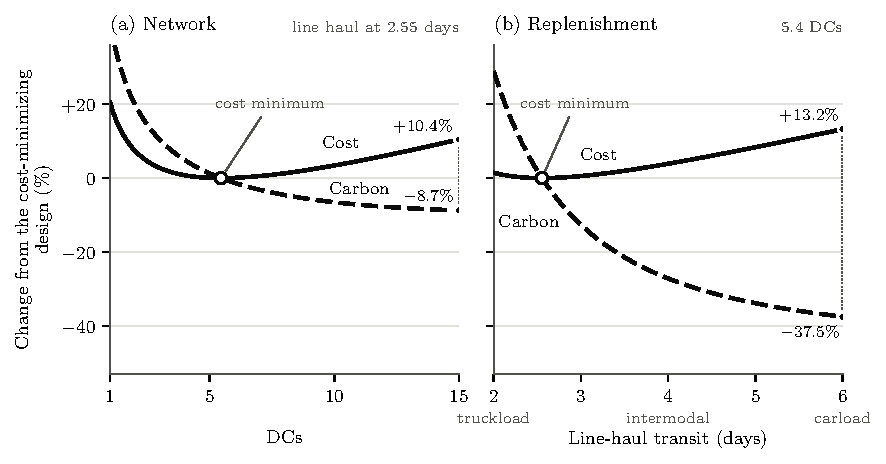
\includegraphics[width=0.91\linewidth]{fig_levers.pdf}
\caption{Annual cost and carbon of the reference network when one decision moves and the other stays at the
cost-minimizing design, which costs $\$97.3$ million and emits $32{,}660$~t a year.}
\label{fig:levers}
\end{figure}

Figure~\ref{fig:levers} shows how annual cost and carbon change when one decision moves away from the
cost-minimizing design and the other is held there. More distribution centers shorten the last-mile legs but add
facility cost and carbon and weaken pooling. At fifteen centers, carbon is $8.7\%$ lower and cost $10.4\%$ higher,
and further centers lower carbon only slightly. Slowing the line haul lowers freight cost and carbon but adds
safety stock and stock in transit, which raise cost and add little carbon. At intermodal's four days, carbon is
$27.1\%$ lower and cost $3.9\%$ higher; at six days, $37.5\%$ lower and $13.2\%$ higher. We next ask how the firm combines the two decisions to
meet a required cut at least cost.

\begin{figure}[t]
\centering
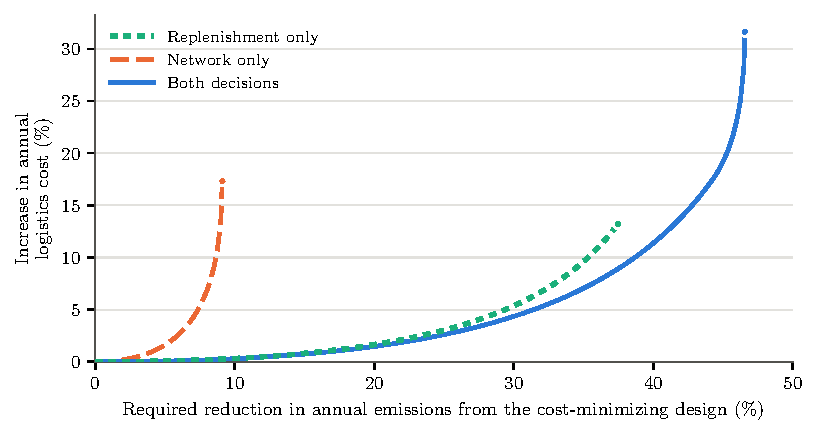
\includegraphics[width=0.86\linewidth]{fig_target.pdf}
\caption{Least-cost design of the reference network for each required cut in emissions, for three sets of
actions. Each curve ends at the largest cut that its actions attain.}
\label{fig:target}
\end{figure}

Figure~\ref{fig:target} traces the least-cost design as the required cut in emissions grows, for three sets of
actions: changing replenishment alone, changing the number of distribution centers alone, and changing both.
Slower line haul delivers most of each cut. At a $20\%$ cut, the least-cost design slows the line haul from $2.55$
to $3.30$ days and grows the network from $5.4$ to $6.2$ centers, at a cost increase of $1.5\%$; lower inbound
freight carbon accounts for $92\%$ of the reduction and shorter store-delivery legs for $10\%$, while added
facility carbon takes back $2\%$. Slowing alone raises cost by $1.6\%$ for the same cut, so changing both
decisions is cheaper, and it also reaches further: slowing alone attains at most a $37.5\%$ cut and adding centers
alone $9.1\%$, whereas changing both attains $46.6\%$, the carbon minimum, with $19.2$ centers and a six-day line
haul. Each cut corresponds to a carbon price (Lemma~\ref{prop:unique}). A $20\%$ cut costs $\$218$ per metric ton
avoided on average and corresponds to a price of $\$542$ per metric ton; both figures price the two design
decisions alone, with fuel, vehicles, and load fill held fixed. A price of $\$100$ per metric ton lowers emissions
by $5.8\%$ at a cost increase of $0.1\%$, and the average metric ton avoided costs $\$48$, less than the price.

\subsection{Robustness}\label{sec:robust}

We examine in Table~\ref{tab:robust} whether the least-cost design for a $20\%$ cut survives changes in the
inputs. Each row reports the cost-minimizing design and the least-cost design for a $20\%$ cut from that row's own
cost minimum; for the caps on realized carbon, the budget is that of the reference row, and demand is independent
across weeks. Every feasible case uses slower replenishment. The network expands under continuous service
choices but contracts slightly when only the three discrete services are available.

\begin{table}[t]
\centering\small
\caption{Least-cost design for a cut of at least $20\%$ in emissions under alternative inputs. Days are line-haul transit
times.}
\label{tab:robust}
\setlength{\tabcolsep}{4pt}
\begin{tabular}{@{}lccccc@{}}
\toprule
 & \multicolumn{2}{c}{Cost minimum} & \multicolumn{3}{c}{Least cost for at least $20\%$ cut}\\
\cmidrule(lr){2-3}\cmidrule(l){4-6}
 & Centers & Days & Centers & Days & Cost increase\\
\midrule
Reference                                     & $5.4$ & $2.55$ & $6.2$  & $3.30$ & $1.5\%$\\
Whole number of centers                       & $5$   & $2.56$ & $6$    & $3.26$ & $1.2\%$\\
Truckload, intermodal, or carload only        & $5.5$ & $2.00$ & $5.4$  & $4.00$ & $2.4\%$\\
\addlinespace
\multicolumn{6}{@{}l}{\itshape Holding cost}\\
Capital charge $10\%$                         & $5.5$ & $2.93$ & $6.5$  & $3.97$ & $1.7\%$\\
Capital charge $25\%$                         & $5.3$ & $2.14$ & $5.8$  & $2.65$ & $1.3\%$\\
Pallet value $\$10{,}000$                     & $5.6$ & $3.24$ & $6.7$  & $4.56$ & $2.0\%$\\
Pallet value $\$50{,}000$                     & $5.1$ & $2.00$ & $5.8$  & $2.43$ & $2.1\%$\\
\addlinespace
\multicolumn{6}{@{}l}{\itshape Line-haul carbon}\\
Efficient diesel truck, $1.34$~kg per mile    & $5.4$ & $2.55$ & $6.6$  & $3.44$ & $2.1\%$\\
Electric truck, $2.0$~kWh per mile            & $5.4$ & $2.55$ & \multicolumn{3}{c}{not attainable; largest cut $18.9\%$}\\
Intermodal $45\%$ below truckload             & $5.4$ & $2.55$ & $7.1$  & $3.72$ & $3.4\%$\\
Intermodal $70\%$ below truckload             & $5.4$ & $2.55$ & $5.9$  & $3.13$ & $0.9\%$\\
\addlinespace
\multicolumn{6}{@{}l}{\itshape Warehouse and store-delivery carbon}\\
Warehouse carbon halved                       & $5.4$ & $2.55$ & $6.2$  & $3.26$ & $1.4\%$\\
Warehouse carbon doubled                      & $5.4$ & $2.55$ & $6.1$  & $3.36$ & $1.6\%$\\
Refrigerated storage                          & $3.5$ & $2.55$ & $4.0$  & $3.45$ & $1.7\%$\\
Electric store delivery, $r_L=0.16$           & $5.4$ & $2.55$ & $5.5$  & $3.14$ & $0.9\%$\\
\addlinespace
\multicolumn{6}{@{}l}{\itshape Carbon accounting}\\
No financing of stock in transit              & $5.4$ & $4.36$ & $9.8$  & $6.00$ & $4.8\%$\\
Annual cap on realized carbon, $95\%$         & $5.4$ & $2.55$ & $6.5$  & $3.51$ & $2.3\%$\\
Weekly cap on realized carbon, $95\%$         & $5.4$ & $2.55$ & $9.2$  & $5.16$ & $11.9\%$\\
\bottomrule
\end{tabular}
\end{table}

With whole centers, the cost minimum has five centers and the design for the cut six, with a line haul of $3.26$
days, at a cost increase of $1.2\%$. With only truckload, intermodal, and carload services, the least-cost design for the cut moves the whole flow
from truckload to intermodal with $5.4$ centers, at $2.4\%$, and overshoots the target with a $43\%$ cut; the line
haul slows, but the network does not grow. 

Holding cost decides where the cost minimum lies on the speed range, and so how much slowing has to give; the
cost-minimizing network itself changes little, between $5.1$ and $5.6$ centers. A higher capital charge or pallet
value makes the cost-minimizing chain faster. At a $25\%$ charge it ships in $2.14$ days, and a cut of $20\%$ takes
$5.8$ centers and $2.65$ days, at $1.3\%$; at $\$50{,}000$ a pallet it ships by truckload, and the cut takes $5.8$
centers and $2.43$ days, at $2.1\%$, because slowing then ties up costlier stock. A lower charge or value makes the
chain slower, $2.93$ days at a $10\%$ charge and $3.24$ days at $\$10{,}000$ a pallet, and the least-cost designs
for the cut have $6.5$ centers and $3.97$ days, at $1.7\%$, and $6.7$ centers and $4.56$ days, at $2.0\%$.

The carbon that slowing saves matters more. These inputs leave cost unchanged, so the cost minimum stays at $5.4$
centers and $2.55$ days. With an efficient diesel truck at $1.34$~kg per mile, slowing saves less carbon, and the
least-cost design for the cut has $6.6$ centers and $3.44$ days, at $2.1\%$; with a battery-electric truck at
about $2$~kWh per mile, the line haul carries so little carbon that the largest attainable cut is $18.9\%$. If
intermodal emits $45\%$ less than truckload, the design has $7.1$ centers and $3.72$ days, at $3.4\%$, and if it
emits $70\%$ less, $5.9$ centers and $3.13$ days, at $0.9\%$.

Warehouse carbon matters less, because transport dominates the network's emissions: with it halved, the design for
the cut has $6.2$ centers and $3.26$ days, at $1.4\%$, and with it doubled, $6.1$ centers and $3.36$ days, at
$1.6\%$. Refrigerated storage doubles the fixed cost of a center, so the network operates $3.5$ centers at the
cost minimum and $4.0$ for the cut, with $3.45$ days, at $1.7\%$. Electric store delivery, whose carbon per dollar
is nearer that of a center, calls for $5.5$ centers and $3.14$ days, at $0.9\%$. Without financing, the
cost-minimizing chain already ships in $4.36$ days, so the cut requires the slowest service and $9.8$ centers, at a
cost increase of $4.8\%$. A cap on realized carbon at the reference budget requires a deeper expected cut: for an
annual cap, $23.8\%$, with $6.5$ centers and $3.51$ days, at $2.3\%$; for a weekly cap, $40.5\%$, with $9.2$ centers
and $5.16$ days, at $11.9\%$.

\section{Managerial Implications}\label{sec:managerial}

In this section, we show how a firm can use its operating rates, demand characteristics, and cost-minimizing
configuration to tell which of its distribution decisions a carbon price will move, in which direction, and by
how much. Each implication follows from a result of Section~\ref{sec:analysis}; the calibrated values of
Section~\ref{sec:numerical} illustrate it.

\paragraph{A diagnostic in two questions.} A firm needs four ratios and two shares. The ratios are the carbon
per dollar of holding stock, of the speed it can buy on its line-haul lane, of last-mile delivery, and of
operating a distribution center. Because labor and capital carry little carbon, a firm can estimate the ratios from its fuel, electricity,
warehousing, and spoilage records (Section~\ref{sec:calib}). The shares
are the pooling weight $\omega$ --- the share of a distribution center's marginal cost that is lost pooling ---
and the safety-stock share $a_K$ of the inventory that speed saves, and the firm can obtain both from its
cost-minimizing network through \eqref{eq:poolweight} and \eqref{eq:stockshare}. Proposition~\ref{prop:classify}
then gives the direction of both decisions, and Table~\ref{tab:regimes} sets out the four combinations; off the diagonal,
the speed direction shown holds whenever $a_KR_{\mathrm{speed}}$ lies outside the bands \eqref{eq:speedbands}.

\begin{table}[t]
\centering\small
\caption{Carbon-minimizing direction of the two decisions (Proposition~\ref{prop:classify}), with examples from Table~\ref{tab:ratios}.}
\label{tab:regimes}
\renewcommand{\arraystretch}{1.25}
\begin{tabular}{@{}>{\raggedright\arraybackslash}p{0.27\linewidth}
                   >{\raggedright\arraybackslash}p{0.32\linewidth}
                   >{\raggedright\arraybackslash}p{0.32\linewidth}@{}}
\toprule
 & \textbf{More distribution centers}\newline {\small\itshape last mile more carbon-intensive per dollar than facilities and lost pooling}
 & \textbf{Fewer distribution centers}\newline {\small\itshape last mile less carbon-intensive per dollar than facilities and lost pooling} \\
\midrule
\textbf{Faster replenishment}\newline {\small\itshape inventory saving from speed more carbon-intensive per dollar than the speed it buys}
  & team drivers for perishables that spoil; diesel delivery
  & team drivers for perishables that spoil; electric vans \\
\textbf{Slower replenishment}\newline {\small\itshape inventory saving from speed less carbon-intensive per dollar than the speed it buys}
  & speed bought with fuel, or team drivers for high-value goods; diesel delivery
  & speed bought with fuel for refrigerated goods; electric vans \\
\bottomrule
\end{tabular}
\end{table}

\paragraph{Slow the speed bought with fuel; buy speed with labor where held stock carries carbon.} A faster
vessel, truck instead of intermodal rail, and air instead of truck add cost that is mostly fuel, so their carbon per
dollar is many times that of holding stock (Table~\ref{tab:ratios}). By Proposition~\ref{prop:speed}, a carbon
price then favors slower replenishment, and financing the goods in transit strengthens that direction because it
lowers the share $a_K$. In the reference network, slower line haul delivers $92\%$ of a $20\%$ cut in emissions
(Figure~\ref{fig:target}). The shifts of pharmaceutical freight from air to ocean and of truckload lanes to
intermodal rail are consistent with this direction \citep{pharmcommerce2023astrazeneca, freightwaves2026intermodal},
as is the finding of \citet{maloni2013slow} that slower vessel speed lowers carbon and total cost despite the
added pipeline inventory. The speed a team of drivers buys costs wages and little fuel, so a carbon price favors it
wherever held stock carries enough carbon that the inventory saving from speed is more carbon-intensive per dollar
than that speed. Measured by site energy, holding ambient packaged goods emits $0.056$~kg per dollar and holding
perishables that spoil $0.46$, about twice and fifteen times the ratio of team operation (Table~\ref{tab:ratios});
in our calibration only perishables that spoil move to team drivers, and for high-value goods, whose holding cost
is mostly capital, a carbon price favors a solo driver. A team shortens lead time only where a trip exceeds the distance one driver may cover in a day, so speed
bought with labor matters most on long lanes.

\paragraph{Reassess network density when delivery technology changes.} The density decision compares the carbon
per dollar of last-mile delivery with that of a distribution center's facility and lost pooling
(Propositions~\ref{prop:density} and~\ref{prop:classify}). Diesel delivery, by truck or van, is carbon-intensive enough per dollar to call for more distribution centers
closer to demand. At the central ratios of Table~\ref{tab:ratios}, so is an electric truck: it emits $0.16$~kg per
dollar against $0.082$ for an ambient center. An electric van emits about as much per dollar as an ambient center,
so for ambient goods the comparison is close to parity; it emits half as much as a refrigerated center, so for cold
chains a carbon price favors fewer, larger centers. In the reference network, we find that a $20\%$ cut takes $5.5$
centers with electric trucks against $6.2$ with diesel trucks (Table~\ref{tab:robust}). Amazon reports that placing inventory closer to customers
avoided $127$ million vehicle miles in 2025 \citep{amazon2025sustainability}, a move in the direction
Proposition~\ref{prop:classify} gives when the last mile is carbon-intensive. A firm that electrifies its last
mile should therefore revisit how many distribution centers it operates. The carbon intensity of the line haul also bears on density, through the share of a carbon target that slowing
can deliver: a $20\%$ cut takes $7.1$ centers when intermodal emits $45\%$ less than truckload and $5.9$ when it
emits $70\%$ less (Table~\ref{tab:robust}).

\paragraph{Expect modest moves at current carbon prices.} By Proposition~\ref{prop:path}, the response to a
carbon price depends on the carbon share of each activity's cost, carbon charge included. At $\$100$ per metric ton,
carbon is under $1\%$ of the cost of holding ambient goods and of operating facilities, $5\%$ of the
cost of diesel truck delivery, $17\%$ of speed bought with truck instead of intermodal rail, and $35\%$ of speed bought with vessel
speed; it reaches half of the cost of diesel truck delivery only at about $\$2{,}000$ per metric ton. In the reference network a price of $\$100$ per metric ton lowers emissions by $5.8\%$ at a cost increase of
$0.1\%$, almost entirely through slower line haul, and a $20\%$ cut, which corresponds to a price of $\$542$ per
metric ton, grows the network from $5.4$ to $6.2$ centers (Figure~\ref{fig:target}). We note in
Section~\ref{sec:path} that the first response of density can run opposite to the carbon-minimizing direction;
in the reference network it does not, because diesel delivery exceeds both thresholds. The two decisions are complements (Lemma~\ref{prop:unique}), so a
program that acts on one alone, such as a slow-steaming mandate or a consolidation drive, evaluates it at a level
of the other decision that the joint design would change.

\paragraph{Account for realized carbon over short horizons.} A cap on realized carbon places
a risk margin on transport emissions (Corollary~\ref{prop:chance}). For a weekly cap held with $95\%$
confidence, the margin raises the transport carbon rates by $37\%$ in our calibration, and for an annual cap by
about $5\%$. In the
reference network, a weekly cap at the expected budget raises the cost of a $20\%$ cut from $1.5$ to $11.9\%$, and
an annual cap to $2.3\%$ (Table~\ref{tab:robust}).

\paragraph{Implications for policy.} An instrument that prices transport carbon alone, such as a freight fuel
levy, blends the carbon price into the transport rates and leaves holding and
facility carbon unpriced. At a given density it therefore slows replenishment, and at a given speed it adds distribution centers, whatever
the product. By Propositions~\ref{prop:speed} and~\ref{prop:density}, these moves raise total carbon, at least
for small prices, when the inventory saving from speed is more carbon-intensive per dollar than the speed it would
buy, or when the last mile is less carbon-intensive per dollar than facilities and lost pooling; when both
decisions adjust, the effect depends on their joint response. By the ratios of Table~\ref{tab:ratios}, the first
condition holds for perishables that spoil served by team drivers and the second for electric vans in cold
chains. An instrument that prices total logistics carbon lets the firm weigh all four activities when it
chooses speed and density.

\section{Discussion and Conclusion}\label{sec:discussion}

A firm that distributes through regional distribution centers provides availability through safety stock or
replenishment speed and proximity through facilities or last-mile travel, and a carbon price or cap can change
which activity provides each. We have shown that the joint design has a unique optimum at every carbon price and that the carbon-minimizing
direction of density, and of speed when the speed and density comparisons agree, follows from four
carbon-intensity-per-dollar ratios and two shares of the cost-minimizing design. In public US data, the classification depends on the product, on how
speed is bought, and on how the last mile is driven. Several documented moves
in practice are consistent with these directions; in the sources we examine, firms report them in terms of cost,
delivery service, and transport miles. Our model adds the carbon of the inventory a slower chain holds, the
financing of the goods it carries, and the link between speed and density.

\paragraph{Limitations.} The model describes an average, symmetric distribution environment, so its
classification serves as a diagnostic for a heterogeneous network. Heterogeneous markets or
discrete facility sites replace $d(n)=\delta n^{-1/2}$ with the realized last-mile profile; this can move the
density threshold but leaves the comparison between facility and last-mile carbon per dollar intact. The representative inbound distance isolates the proximity effect of adding distribution centers. If more centers also
mean smaller inbound shipments or lower vehicle fill, those forces favor consolidation and
can move a case near the threshold. We charge the financing of goods in transit to the firm that owns them; a firm that buys on delivered terms may
still bear that cost through the supplier's price. We treat speed as a continuous index between real options on
a lane, and we assume that all inbound volume can use each option; where only part of it can move by rail,
slowing reaches a smaller share of emissions. Carload transit times also vary more than intermodal's
\citep{kwon1995trip}, and the model, which treats transit time as fixed, does not price that variability. A firm that splits volume between modes
faces a mixture of lead times, and our safety-stock expression does not represent such a mixture. The model ties last-mile distance to the number of
stocking distribution centers, whereas networks that deliver through cross-docks or hubs separate stocking density
from delivery density. Service enters as a cycle-service requirement; if it is chosen, safety stock becomes a
further design margin. Finally, we calibrate the carbon intensities to public industry data, so a firm should compute the
classification with its own rates, and the magnitudes in
Section~\ref{sec:numerical} describe the network we calibrate.

\paragraph{Future research.} Future research could extend the model to multi-product and multi-echelon settings,
where a shared network serves products in different regimes and safety stock can be held at more than one
echelon. Separating stocking from delivery density,
and modeling shipment consolidation and routing explicitly, would quantify these centralizing forces. As accounting under ISO 14083 makes firm-level logistics-emissions data available \citep{iso2023_14083}, empirical
work can locate real products relative to the speed and density thresholds.
Endogenous service choice and explicit mode mixes are natural extensions.

\section*{Data availability}

\noindent The data and code supporting the numerical illustrations are available from the author on reasonable
request.

\bibliographystyle{apalike}
\bibliography{references}

\appendix
\section{Proofs}\label{app:proofs}

\begin{proof}[Proof of Lemma~\ref{prop:unique}]
We give the argument for $J$; for $C$ replace each blended rate by its carbon rate and set $h_p=0$. Let $x=\ln n$ and $y=\ln v$,
which range over a box, and let $k=z\sigma\sqrt{ND}$. Then, up to the constant $cN\mu$,
\[
  J=F_\tau e^{x}+H_\tau k\,e^{g(x,y)}+h_pN\mu D\,e^{-y}+T_\tau(e^{y})\,N\mu D+\ell_\tau N\mu\delta\,e^{-x/2},
\]
with $g(x,y)=\tfrac12\ln\big(N\rho+(1-\rho)e^{x}\big)-\tfrac12y$.
(i) The facility and last-mile terms are strictly convex in $x$. The function $g$ is convex, because
$\ln(c_1+c_2e^{x})$ is convex for $c_1\ge0$ and $c_2>0$, so the holding term is log-convex and therefore convex. The
transport term is convex in $y$, because $T_\tau$ is convex and nondecreasing and $e^{y}$ is convex. For strict
convexity, let $S=H_\tau k\,e^{g}$; its Hessian is $S\big(\nabla^2g+\nabla g\,\nabla g^{\mathsf T}\big)$, with
$\nabla g=(g_x,-\tfrac12)$ and $\nabla^2g=\mathrm{diag}(g_{xx},0)$, $g_{xx}\ge0$. The Hessian of the facility,
holding, and last-mile terms therefore has $(x,x)$ entry
$F_\tau e^{x}+\tfrac14\ell_\tau N\mu\delta e^{-x/2}+S(g_{xx}+g_x^2)>0$, $(y,y)$ entry $S/4$, and off-diagonal
entry $-Sg_x/2$, so its determinant is $\big(F_\tau e^{x}+\tfrac14\ell_\tau N\mu\delta e^{-x/2}\big)S/4+S^2g_{xx}/4>0$.
Adding the convex transport and financing terms preserves strict convexity.
(ii) A strictly convex continuous function has a unique minimizer on a compact convex set. Since $J$ is continuous
in $(x,y,\tau)$, the minimizer is continuous in $\tau$ by the maximum theorem.
(iii) For fixed $x$, $J$ is strictly convex in $y$, so the speed response is unique and, by the maximum theorem,
continuous. Only the holding term couples $x$ and $y$, with cross-partial $-Sg_x/2\le0$, so $J$ has decreasing
differences in $(x,y)$ and each response is nondecreasing in the other decision. The reduced objective, the partial
minimum of a strictly convex function over a convex set, is strictly convex in $x$ and so strictly quasiconvex in
$n$; by Danskin's theorem, which applies because the speed response is unique,
$J^{\mathrm r}_n(n)=J_n\big(n,v^*(n)\big)$, which changes sign at most once, from negative to positive. For strict
monotonicity with $\rho<1$: where $v^*$ is interior, the right side of \eqref{eq:focv} strictly increases in $n$
and strictly decreases in $v$, while its left side does not depend on $n$ and is nondecreasing in $v$, so $v^*$
strictly increases in $n$, and projection onto the speed bounds preserves monotonicity. Since
$J_{nv}=-H_\tau G(n,v)/(2v)<0$, the sign change of $J_n(\cdot,v)$ occurs at a higher $n$ when $v$ rises.
\end{proof}

\begin{proof}[Proof of Proposition~\ref{prop:speed}]
(i) $N\mu D\,t(v)$, $N\mu D\,\varepsilon(v)$, and $h_pN\mu D\,v^{-1}$ are convex and $\kappa(n)v^{-1/2}$ has
$\partial_v^2=\tfrac34 \kappa(n)v^{-5/2}>0$, so both objectives are strictly convex in $v$. We use
$M_s=\tfrac12 h\,\kappa(n)\,v_{\mathrm K}^{-3/2}=h\sstock/(2v_{\mathrm K})$ and
$M_p=h_pN\mu D\,v_{\mathrm K}^{-2}=h_pP/v_{\mathrm K}$ to denote the marginal savings of safety stock and of stock
in transit, so that $a(n,v_{\mathrm K})=M_s/(M_s+M_p)$. The cost optimum
satisfies $\hat K'(v_{\mathrm K})=0$, i.e.\ $N\mu D\,t'(v_{\mathrm K})=M_s+M_p$, so that
$\tfrac12 \kappa(n)v_{\mathrm K}^{-3/2}=a(n,v_{\mathrm K})\,N\mu D\,t'(v_{\mathrm K})/h$. Evaluating the carbon
derivative there,
\[
  \hat C'(v_{\mathrm K})=-\eta\,\tfrac12 \kappa(n)v_{\mathrm K}^{-3/2}+N\mu D\,\varepsilon'(v_{\mathrm K})
  =N\mu D\big(\varepsilon'(v_{\mathrm K})-a(n,v_{\mathrm K})\,(\eta/h)\,t'(v_{\mathrm K})\big),
\]
which is negative --- so $v_C>v_{\mathrm K}$ by strict convexity --- if and only if \eqref{eq:speedthreshold}.
With $t'=2t_1 v$ and $\varepsilon'=2\varepsilon_0 v$ the marginal ratio is $\varepsilon_0/t_1$, and with $h_p=0$
the priced first-order condition \eqref{eq:focv} gives
$v^{5/2}=(h+\tau\eta)z\sigma\sqrt{ND}\,\sqrt{\Psi}/[4(t_1+\tau\varepsilon_0)N\mu D]$, which is
\eqref{eq:vstar}. The projection and the boundary qualification are immediate.
(ii) Let $s=z\sigma$, so that $\sstock\propto s\,v^{-1/2}$. Under the quadratic instantiation, condition
\eqref{eq:focv} takes the form $M_s+M_p=2(t_1+\tau\varepsilon_0)N\mu D\,v$ with $M_s=H_\tau\sstock/(2v)\propto
s\,v^{-3/2}$ and $M_p=h_pN\mu D\,v^{-2}$; let $a_\tau=M_s/(M_s+M_p)$. Implicit differentiation gives
$\mathrm d\ln v^*/\mathrm d\ln s=M_s/(\tfrac52M_s+3M_p)=a_\tau/(3-a_\tau/2)\in(0,\tfrac25]$, so speed rises with
service and demand volatility; without financing $v^*\propto s^{2/5}$, as in \eqref{eq:vstar}. At $\tau=0$,
$M_s/M_p\propto s\,v_{\mathrm K}^{1/2}$ rises in $s$, directly and through $v_{\mathrm K}$, so $a(n,v_{\mathrm K})$
rises in $s$; the right side of \eqref{eq:speedthreshold} is the constant $\varepsilon_0/t_1$, so the comparison
can change only toward faster replenishment, and without financing it does not change.
\end{proof}

\begin{proof}[Proof of Proposition~\ref{prop:density}]
(i) By Lemma~\ref{prop:unique}(iii), $J(\cdot,v)$ and $C(\cdot,v)$ are strictly quasiconvex on $[1,N]$, which
gives uniqueness and the interior/boundary characterization. For the threshold, take $\tau=0$ for cost and
$\tau\to\infty$ for carbon. The cost density satisfies $\partial_n K=F+h\,G(n_K,v)-
t_L N\mu\delta/(2n_K^{3/2})=0$, so the last-mile marginal $t_L N\mu\delta/(2n_K^{3/2})=F+h\,G(n_K,v)$.
Evaluating the carbon derivative there,
\[
  \partial_n C\big|_{n_K}
  =\varphi+\eta\,G(n_K,v)-\frac{\varepsilon_L N\mu\delta}{2n_K^{3/2}}
  =\varphi+\eta\,G(n_K,v)-\frac{\varepsilon_L}{t_L}\,\big[F+h\,G(n_K,v)\big],
\]
which is negative --- so $n_C>n_K$ by strict quasiconvexity of $C(\cdot,v)$ --- if and only if
\eqref{eq:densthreshpool}. With $R(G)=(\varphi+\eta G)/(F+hG)$, we have $R(0)=\varphi/F$, $R(G)\to\eta/h$ as $G\to\infty$, and
$R'(G)=(\eta F-h\varphi)/(F+hG)^2$, so $R$ is monotone with $\operatorname{sign}R'=\operatorname{sign}
(\eta/h-\varphi/F)$ and lies between $\varphi/F$ and $\eta/h$. In the no-pooling limit $\rho\to1$, $G\to0$ and $\Psi\to N$, so
\eqref{eq:focn} gives $n^*=(\ell_\tau N\mu\delta/2F_\tau)^{2/3}$ and \eqref{eq:densthreshpool} becomes \eqref{eq:densitythreshold}.
(ii) Along the speed response of Proposition~\ref{prop:speed}(ii), $J^{\mathrm r}_n(n;s)=J_n\big(n,v^*(n;s);s\big)$
because $J_v=0$. The holding marginal term in \eqref{eq:focn} is proportional to
$s(v^*)^{-1/2}(1-\rho)/\sqrt{\Psi(n)}$, whose elasticity in $s$ is $1-a_\tau/(6-a_\tau)\ge\tfrac45$, so it rises in
$s$ even after the induced speed increase, and $J^{\mathrm r}_{ns}>0$. By Lemma~\ref{prop:unique}(iii),
$J^{\mathrm r}_n(\cdot\,;s)$ changes sign at most once, from negative to positive, and it is increasing in $s$; its
sign change therefore occurs at a lower $n$ when $s$ rises, so the optimal density is nonincreasing in $s$, and
strictly decreasing where it is interior.
\end{proof}

\begin{proof}[Proof of Proposition~\ref{prop:classify}]
(i) By Lemma~\ref{prop:unique} applied to the carbon objective, $n_C>n_K$ if and only if the reduced
carbon objective slopes downward at $n_K$, $C^{\mathrm r}_n(n_K)<0$, and $n_C=n_K$ if it is zero. By the
envelope theorem (Danskin's theorem, since $\hat v_C$ is unique whether or not it is at a bound),
$C^{\mathrm r}_n(n_K)=\varphi+\eta\,G(n_K,\hat v_C)-\tfrac12\varepsilon_LN\mu\delta\,n_K^{-3/2}$. The cost condition \eqref{eq:focn} at $\tau=0$, which holds because $n_K$ is
interior, gives $\tfrac12t_LN\mu\delta\,n_K^{-3/2}=F+hG(n_K,v_K)$, and the last term equals
$r_L\big[F+hG(n_K,v_K)\big]$. Since $G\propto v^{-1/2}$, $\eta\,G(n_K,\hat v_C)=h\,G(n_K,v_K)\,r_h\sqrt{v_K/\hat v_C}$.
Dividing $C^{\mathrm r}_n(n_K)$ by $F+hG(n_K,v_K)>0$ and substituting $\varphi=F\,r_F$ gives \eqref{eq:jointdensgen}.
Under the quadratic instantiation with $v_K$ and $\hat v_C$ interior, the carbon condition \eqref{eq:focv} at
$n_K$ gives $\eta\sstock(n_K,\hat v_C)=4\varepsilon_0N\mu D\,\hat v_C^2$, and the cost condition gives
$h\sstock(n_K,v_K)=4a_Kt_1N\mu D\,v_K^2$; with $\sstock\propto v^{-1/2}$ these imply
$(\hat v_C/v_K)^{5/2}=a_KR_{\mathrm{speed}}$, so $r_h\sqrt{v_K/\hat v_C}=r_h^{4/5}r_t^{1/5}a_K^{-1/5}$, which is
\eqref{eq:jointdens}. The second expression for $\omega$ in \eqref{eq:poolweight} follows from
$F+hG(n_K,v_K)=\tfrac12t_LN\mu\delta\,n_K^{-3/2}$ and $F=\tfrac12t_LN\mu\delta\,(n_K^0)^{-3/2}$.
(ii) The carbon objective has no financing term, so by \eqref{eq:focv} its speed response satisfies
$v_C(n)^{5/2}\propto\sqrt{\Psi(n)}$, and $\ln[v_C/\hat v_C]=\tfrac15\ln[\Psi(n_C)/\Psi(n_K)]$. Adding
$\ln[\hat v_C/v_K]=\tfrac25\ln(a_KR_{\mathrm{speed}})$ from part (i) gives \eqref{eq:speeddecomp}. If
\eqref{eq:jointdens} holds and $a_KR_{\mathrm{speed}}\ge1$, then $n_C>n_K$ and $\Psi(n_C)>\Psi(n_K)$, so in
\eqref{eq:speeddecomp} the first term
is nonnegative and the second positive; the reversed case is symmetric. Since $\Psi$ is increasing with
$\Psi(1)\le\Psi(n_C)\le\Psi(N)=N$, the threshold $\sqrt{\Psi(n_K)/\Psi(n_C)}$ lies in $[\underline R,\overline R]$.
(iii) With $\rho=1$, $\Psi\equiv N$ and $G\equiv0$, so \eqref{eq:focn} involves only $F_\tau$ and $\ell_\tau$ and
gives $n^*(\tau)=(\ell_\tau N\mu\delta/2F_\tau)^{2/3}$; the ratio of its carbon and cost values is
$(r_L/r_F)^{2/3}$. The speed response no longer depends on $n$, and
by the argument of part (i) the ratio of its carbon and cost values is $(a_KR_{\mathrm{speed}})^{2/5}$. For
\eqref{eq:excess}, carbon separates into a proximity component $C_{\mathrm{prox}}(n)=\varphi n+\varepsilon_LN\mu
\delta n^{-1/2}$, an availability component $C_{\mathrm{avail}}(v)=\eta z\sigma N\sqrt{D/v}+\varepsilon_0N\mu
D\,v^2$, and the constant $\varepsilon_bN\mu D$, with $\theta=C_{\mathrm{prox}}(n_C)/C_{\min}$ and
$\theta_a=C_{\mathrm{avail}}(v_C)/C_{\min}$. A function $c_1n+c_2n^{-1/2}$ attains its minimum
$3c_1n^\circ$ at $n^\circ=(c_2/2c_1)^{2/3}$ and equals $c_1n^\circ(x+2x^{-1/2})$ at $n=xn^\circ$; with $n_K=xn_C$
and $x=R_{\mathrm{density}}^{-2/3}$, $C_{\mathrm{prox}}(n_K)/C_{\mathrm{prox}}(n_C)=(x+2x^{-1/2})/3$. Likewise
$c_1v^{-1/2}+c_2v^2$ attains its minimum $\tfrac54c_1(v^\circ)^{-1/2}$ and equals
$c_1(v^\circ)^{-1/2}(y^{-1/2}+y^2/4)$ at $v=yv^\circ$, so with $v_K=yv_C$ and
$y=(a_KR_{\mathrm{speed}})^{-2/5}$, $C_{\mathrm{avail}}(v_K)/C_{\mathrm{avail}}(v_C)=(4y^{-1/2}+y^2)/5$. Weighting by
$\theta$ and $\theta_a$ and adding the constant share $1-\theta-\theta_a$ gives $C(n_K,v_K)/C_{\min}$ exactly.
Expanding $x=e^{u_1}$ and $y=e^{u_2}$ to second order gives \eqref{eq:excess}.
\end{proof}

\begin{proof}[Proof of Proposition~\ref{prop:path}]
(i) Condition \eqref{eq:focv} is $\Upsilon(v,\tau)=2b_\tau N\mu D\,v-M_s-M_p=0$, with $b_\tau=t_1+\tau\varepsilon_0$,
$M_s=H_\tau\sstock/(2v)$, and $M_p=h_pP/v$. Then $v\,\Upsilon_v=\tfrac52M_s+3M_p$ and, since
$\tau\eta/H_\tau=s_h$ and $\tau\varepsilon_0/b_\tau=s_t$, $\tau\,\Upsilon_\tau=s_t(M_s+M_p)-s_hM_s$. Hence
$\mathrm d\ln v^*/\mathrm d\ln\tau=-\tau\Upsilon_\tau/(v\Upsilon_v)=(a_\tau s_h-s_t)/(3-a_\tau/2)$ with $a_\tau=M_s/(M_s+M_p)$.
Substituting the definitions, $a_\tau s_h-s_t=\tau\,(h\sstock+2h_pP)\,t_1\,[a(n,v^*)\,r_h-r_t]/
[(H_\tau\sstock+2h_pP)\,b_\tau]$, which has the sign of $a(n,v^*)r_h-r_t$. Because $a(n,v)$ rises with $v$, a
positive sign raises $v^*$ and keeps the sign positive, and a negative sign lowers $v^*$ and keeps it negative, so
the sign does not change along the path and $v^*$ is monotone in $\tau$. With $h_p=0$, $a_\tau=1$ and the
elasticity is $\tfrac25(s_h-s_t)$. (ii) The same computation
applies to $n^*=(\ell_\tau N\mu\delta/2F_\tau)^{2/3}$. (iii) With $h_p=0$, by \eqref{eq:vstar}, along the speed response
$H_\tau G\big(n,v^*(n)\big)=c_G\,(1-\rho)\,H_\tau^{4/5}b_\tau^{1/5}\Psi(n)^{-3/5}$, with $b_\tau=t_1+\tau\varepsilon_0$
and $c_G>0$ depending on neither $n$ nor $\tau$. By the envelope theorem, $J^{\mathrm r}_n=F_\tau+H_\tau G\big(n,v^*(n)\big)-\tfrac12\ell_\tau N\mu\delta n^{-3/2}$;
multiplying by $n^{3/2}/\ell_\tau>0$ preserves its sign,
\[
  \frac{n^{3/2}J^{\mathrm r}_n}{\ell_\tau}=\frac{F_\tau}{\ell_\tau}\,n^{3/2}
  +c_G\,(1-\rho)\,\frac{H_\tau^{4/5}b_\tau^{1/5}}{\ell_\tau}\,\frac{n^{3/2}}{\Psi(n)^{3/5}}-\tfrac12N\mu\delta .
\]
This expression changes sign at most once, from negative to positive (Lemma~\ref{prop:unique}(iii)). If
both coefficients are nonincreasing in $\tau$, the expression is pointwise nonincreasing in $\tau$, so its sign
change moves weakly to higher $n$ and $n^*(\tau)$ is nondecreasing. The logarithmic derivatives of
the coefficients are $1/(r_F^{-1}+\tau)-1/(r_L^{-1}+\tau)$ and
$\tfrac45/(r_h^{-1}+\tau)+\tfrac15/(r_t^{-1}+\tau)-1/(r_L^{-1}+\tau)$. Since $1/(r^{-1}+\tau)$ is increasing in
$r$, both are nonpositive at every $\tau$ when $r_L$ exceeds $r_F$, $r_h$, and $r_t$, and nonnegative when it
falls short of each.

\emph{Low-price density response \eqref{eq:lowprice}.} In $x=\ln n$ and $y=\ln v$, with subscripts denoting
partial derivatives and $S$ and $P$ the safety stock and stock in transit at the interior cost minimum, the Hessian
of $K$ is positive definite (Lemma~\ref{prop:unique}), so differentiating the stationarity
conditions of $K+\tau C$ at $\tau=0$ gives $\operatorname{sign}\mathrm dx^*/\mathrm d\tau=\operatorname{sign}
(K_{xy}C_y-K_{yy}C_x)$. With $M=nF+hSg_x$ the marginal cost of an additional center in logarithmic units, so that
$\omega=hSg_x/M$ and, by $K_x=0$, $M=\tfrac12t_LN\mu\delta n^{-1/2}$, we have $C_x=M[(1-\omega)r_F+\omega
r_h-r_L]$ and $K_{xy}=-\tfrac12\omega M$. The speed condition $K_y=0$ gives $2t_1v^2N\mu D=\tfrac12hS+h_pP=hS/(2a_K)$,
so $K_{yy}=\tfrac14hS+h_pP+4t_1v^2N\mu D=hS(6-a_K)/(4a_K)$ and $C_y=-\tfrac12\eta S+2\varepsilon_0v^2N\mu
D=hS(r_t-a_Kr_h)/(2a_K)$. Substituting, $K_{xy}C_y-K_{yy}C_x>0$ if and only if \eqref{eq:lowprice} holds.
\end{proof}

\begin{proof}[Proof of Corollary~\ref{prop:chance}]
(i) In \eqref{eq:Ctilde} the throughput coefficient $\gamma(n,v)=\varepsilon(v)D+\varepsilon_L d(n)>0$, so
$\{\tilde C\le B\}=\{Q\le(B-\varphi n-\eta\sstock)/\gamma\}$, and $\Pr\{\tilde C\le B\}\ge 1-\beta_c$ holds iff
$(B-\varphi n-\eta\sstock)/\gamma\ge q_{1-\beta_c}$, with $q_{1-\beta_c}=\inf\{q:\Pr(Q\le q)\ge1-\beta_c\}$, i.e.\
$\varphi n+\eta\sstock+\gamma\,q_{1-\beta_c}\le B$. Because
$\gamma\,q_{1-\beta_c}=(q_{1-\beta_c}/N\mu)\,[\varepsilon(v)N\mu D+\varepsilon_L N\mu d(n)]$, this condition is
\eqref{eq:chancecap}. Under normality $q_{1-\beta_c}=N\mu+z_{\beta_c}\sigma_Q$, so $m=1+z_{\beta_c}\,\mathrm{CV}_Q$.
From $\sigma_Q^2=\sigma^2N[1+(N-1)\rho]$, $\mathrm{CV}_Q=(\sigma/\mu)\sqrt{[1+(N-1)\rho]/N}$ is increasing in
$\sigma/\mu$ and, for $N>1$, in $\rho$, and $z_{\beta_c}$ is increasing in $1-\beta_c$, so, for $\beta_c<\tfrac12$, $m$ is increasing in all
three.
(ii) The chance constraint multiplies the inbound and last-mile carbon rates by $m$ and leaves the cost rates,
and so $n_K$, $\omega$, and $a_K$, unchanged; substituting $m\varepsilon_0$ and $m\varepsilon_L$ for
$\varepsilon_0$ and $\varepsilon_L$ in Propositions~\ref{prop:speed}--\ref{prop:classify} gives the thresholds. For the joint speed, divide the carbon density condition by $m$: its facility and
lost-pooling terms then scale as $m^{-1}$ and $m^{-4/5}$ and, multiplied by $n^{3/2}$, rise in $n$ with
elasticities $\tfrac32$ and at least $\tfrac9{10}$, so that, at an interior $n_C$,
$\mathrm d\ln n_C/\mathrm d\ln m\le\tfrac89$. Since $\Psi$ has elasticity at most one in $n$,
\eqref{eq:speeddecomp} with $a_KR_{\mathrm{speed}}/m$ in place of $a_KR_{\mathrm{speed}}$ gives
$\mathrm d\ln v_C/\mathrm d\ln m\le-\tfrac25+\tfrac15\cdot\tfrac89<0$.
\end{proof}

\section{Economies of scale in operating a center}\label{app:scale}

Here we let a center's cost and carbon show economies of scale in its throughput. Each center is sized to its planned
throughput $q=N\mu/n$; its cost is $F+c(q)$ and its carbon $\varphi+\psi(q)$, with $c(q)=c_0(q/q_0)^{\zeta_c}$ and
$\psi(q)=\psi_0(q/q_0)^{\zeta_\psi}$, where $q_0$ is a reference throughput and $\zeta_c,\zeta_\psi\in[0,1]$. An
exponent below one represents economies of scale, and an exponent of one gives the proportional handling of
Section~\ref{sec:model}. The network's
facility cost and carbon are $K_F(n)=Fn+n\,c(N\mu/n)$ and $C_F(n)=\varphi n+n\,\psi(N\mu/n)$, and an additional
center costs and emits
\[
  \bar F=K_F'(n)=F+(1-\zeta_c)\,c(q),\qquad \bar\varphi=C_F'(n)=\varphi+(1-\zeta_\psi)\,\psi(q),
\]
its fixed charge plus the scale economies that the network forgoes by spreading its throughput over one more
center. For exponents between zero and one, $\bar F$ and $\bar\varphi$ fall as the network grows.

Since $n\,c(N\mu/n)=c_0(N\mu/q_0)^{\zeta_c}n^{1-\zeta_c}$, and likewise for $\psi$, the priced facility term
$K_F+\tau C_F$ is a sum of nonnegative multiples of $e^{x}$, $e^{(1-\zeta_c)x}$, and $e^{(1-\zeta_\psi)x}$ in
$x=\ln n$, with second derivative at least $(F+\tau\varphi)e^{x}>0$. The Hessian argument of
Lemma~\ref{prop:unique} therefore goes through, and \eqref{eq:focn} holds with $F_\tau$ replaced by
$\bar F_\tau=\bar F+\tau\bar\varphi$. Propositions~\ref{prop:density} and~\ref{prop:classify}(i)--(ii), and condition
\eqref{eq:lowprice} hold with $F$, $\varphi$, and $r_F$ replaced by $\bar F$,
$\bar\varphi$, and $\bar\varphi/\bar F$, evaluated at the density in question. The closed forms that use $F$
directly, the no-pooling optimum $n^*=(\ell_\tau N\mu\delta/2F_\tau)^{2/3}$, the second expression for $\omega$ in
\eqref{eq:poolweight}, and Proposition~\ref{prop:classify}(iii), hold for the linear model only.

In the no-pooling limit, the density elasticity of Proposition~\ref{prop:path}(ii) becomes
$\mathrm d\ln n^*/\mathrm d\ln\tau=(s_L-\bar s_F)/(\tfrac32-\epsilon_F)$, where $\bar s_F=\tau\bar\varphi/\bar
F_\tau$ is the carbon share of the priced marginal facility cost and
$\epsilon_F=-\mathrm d\ln\bar F_\tau/\mathrm d\ln n=[\zeta_c(1-\zeta_c)c(q)+\tau\zeta_\psi(1-\zeta_\psi)\psi(q)]/\bar
F_\tau$ is the rate at which it falls with density. Differentiating the logarithm of $\bar
F_\tau(n)=\tfrac12\ell_\tau N\mu\delta n^{-3/2}$ gives $\bar s_F-\epsilon_F\,\mathrm d\ln n^*/\mathrm d\ln\tau=
s_L-\tfrac32\,\mathrm d\ln n^*/\mathrm d\ln\tau$, and since $\zeta_c,\zeta_\psi\le1$,
$0\le\epsilon_F\le(\bar F_\tau-F-\tau\varphi)/\bar F_\tau<1$. Economies of scale therefore amplify the local
response of density to a given difference in carbon shares, provided the optimum remains interior. In part (iii),
the facility term of $n^{3/2}J^{\mathrm r}_n/\ell_\tau$ becomes $[F+\tau\varphi+(1-\zeta_c)c(q)+\tau(1-\zeta_\psi)
\psi(q)]\,n^{3/2}/\ell_\tau$. Its throughput part consists of terms in $n^{3/2-\zeta_c}$ and $n^{3/2-\zeta_\psi}$,
so the expression still changes sign at most once, and its derivative in $\tau$ has the sign of
$t_L(1-\zeta_\psi)\psi(q)-\varepsilon_L(1-\zeta_c)c(q)$. The density is therefore nondecreasing along the path if,
in addition to the conditions of part (iii) with $\varphi/F$ in place of $r_F$, $(1-\zeta_\psi)\psi(q)\le
r_L(1-\zeta_c)c(q)$ at every density, and nonincreasing under the reverse inequalities.

Under a cap on realized carbon, centers sized to their planned throughput keep facility carbon deterministic, and
Corollary~\ref{prop:chance} holds with $C_F(n)$ in place of $\varphi n$ and the replacements above. In the
proof of part (ii), the facility
term of the scaled carbon density condition, multiplied by $n^{3/2}$, rises in $n$ with elasticity
$\tfrac32-\epsilon_\varphi>\tfrac12$, where $\epsilon_\varphi=-\mathrm d\ln\bar\varphi/\mathrm d\ln n<1$, so
$\mathrm d\ln n_C/\mathrm d\ln m<2$ and $\mathrm d\ln v_C/\mathrm d\ln m<-\tfrac25+\tfrac15\cdot2=0$. Energy that varied with realized volume would scale by $m^{\zeta_\psi}$.

\end{document}
